\documentclass[8pt,leqno]{beamer}

%%%%%%%%%%%%%%%%%%%%%%%% SET UP ENVIRONMENT ETC %%%%%%%%%%%%%%%%%%%%%%

\mode<presentation>
{
  \usetheme[]{} %Boadilla
% or ...
%	\useoutertheme[height=0pt,width=35pt]{sidebar}
%   \setbeamercolor{sidebar}{bg=gray!95!green}

  \setbeamercovered{transparent}
% or whatever (possibly just delete it)
}

\setbeamertemplate{navigation symbols}{}
%\usefonttheme[onlymath]{serif}
%\usefonttheme{professionalfonts}%[stillsansseriflarge]
\usepackage[english]{babel}
\usepackage[latin1]{inputenc}
\usepackage{fancybox}
\usepackage{xcolor}
%\usepackage{avant}
%\usepackage{cmbright}
\usepackage[T1]{fontenc}
\usepackage{fontawesome}
\usepackage{soul}
\setbeamercovered{dynamic}
\setbeamercolor{normal text}{fg=red!50!green!50!blue}
\setbeamercolor{alerted text}{fg=red!20!green!20!blue}


\setbeamercolor{structure}{fg=red!50!green!50!blue}

%\usepackage{fixpauseincludegraphics}
\usefonttheme{professionalfonts}
\usefonttheme{serif}
%\usepackage{fontspec}
%\setmainfont{Helvetica Neue}
\usepackage{times}
\usepackage{fontawesome}  % this package provides the Twitter logo, if needed
%\usecolortheme[RGB={100,100,150}]{structure}
\setbeamertemplate{blocks}[rounded][shadow=true]
%\setbeamertemplate{background canvas}[vertical shading][bottom=black!10,top=white!100]
\usepackage{setspace}
\usepackage{media9}
%\usepackage{movie15}
\usepackage{animate}
\usepackage{ifthen}
\usepackage{graphicx}
\usepackage{verbatim}
\usepackage{fancyvrb}
\usepackage{listings}
\usepackage{pdfpages}
\usepackage{hyperref}
%\lstset{language=bash}
%\usepackage{xcolor,verbatimbox}
%\usepackage{verbatimbox}
%\usepackage{verbdef}
%\usepackage{lipsum} % just for the example
%\usepackage{framed}
%\usepackage[framemethod=TikZ]{mdframed}
\usepackage[skins]{tcolorbox}
\usepackage[percent]{overpic}


%%%%%%%%%%%%%%%%%%%%%%%% SET UP TITLE / AUTHORS ETC %%%%%%%%%%%%%%%%%%%%%%


\vspace*{0.75cm}
\title[\textcolor{gray}{\textbf{Modelling and data analysis `Winter School'}}] 
{\textcolor{white}{\Huge{Modelling and data analysis\\`Winter School'}}}

%
%\subtitle
%{} % (optional)

\vspace*{-0.125cm}
%\author[\textcolor{gray}{\faTwitter \hspace*{0.15cm} @nick\_golledge}] 
%{\textcolor{white}{\large{\faTwitter \hspace*{0.15cm} @nick\_golledge\inst{1}}\\\vspace*{0.0cm}
%
%\vspace*{0.125cm}
\author[\textcolor{gray}{}]{\textcolor{white}{Nick Golledge\inst{1}, \\
Liz Keller\inst{1,2},\\
Alex Gossart\inst{1},\\
Alena Malyarenko\inst{3},\\
Angela Bahamondes-Dominguez\inst{3},\\
Mario Krapp\inst{2},\\
Dan~Lowry\inst{2},\\
Stefan~Jendersie\inst{1}\\
%
%
}}


\normalsize
\institute[\textcolor{gray}{}] % (optional, but mostly needed)
{\textcolor{white}{
\inst{{1}}{Antarctic Research Centre, Victoria University of Wellington, New Zealand}\\
\inst{{2}}{GNS Science, Lower Hutt, New Zealand}\\
\inst{{3}}{NIWA, Wellington, New Zealand}\\
}


  \vspace*{1.2cm}


}
 
% - Use the \inst command only if there are several affiliations.
% - Keep it simple, no one is interested in your street address.

\date[\textcolor{gray}{}] % (optional)
{\vspace*{-4cm}


%%%%%%%%%%%%%%%%%%%%%%%% ADD SOME LOGOS %%%%%%%%%%%%%%%%%%%%%%


%\begin{columns}
%\column{2cm}
%\column{7cm}
\hspace*{-0.9cm} 
\includegraphics[height=1cm]{./logos/ASP_Hub_COL_black.png}\hspace*{0.2cm} 
\includegraphics[height=1cm]{./logos/VUW-logo-new.jpg}
\hspace*{0.0cm} 
\includegraphics[height=1cm]{./logos/mbie-logo.png} 
\hspace*{0.0cm} 
\includegraphics[height=1cm]{./logos/GNS_logo.jpg}
\hspace*{0.2cm} 
\includegraphics[height=1cm]{./logos/niwa-logo.png}
%\end{columns}
}

%%%%%%%%%%%%%%%%%%%%%%%% SET UP TEMPLATE HEAD / FOOT %%%%%%%%%%%%%%%%%%%%%%


\makeatletter
\setbeamertemplate{footline}
{
  \leavevmode%
  \hbox{%
  \begin{beamercolorbox}[wd=.333333\paperwidth,ht=2.25ex,dp=1ex,center]{author in head/foot}%
    \usebeamerfont{author in head/foot}\insertshortauthor~~\beamer@ifempty{\insertshortinstitute}{}{\insertshortinstitute}
  \end{beamercolorbox}%
  \begin{beamercolorbox}[wd=.333333\paperwidth,ht=2.25ex,dp=1ex,center]{title in head/foot}%
    \usebeamerfont{title in head/foot}\insertshorttitle
  \end{beamercolorbox}%
  \begin{beamercolorbox}[wd=.333333\paperwidth,ht=2.25ex,dp=1ex,right]{date in head/foot}%
    \usebeamerfont{date in head/foot}\insertshortdate{}\hspace*{2em}
    \insertframenumber{} / \inserttotalframenumber\hspace*{2ex} 
  \end{beamercolorbox}}%
  \vskip0pt%
}
\makeatother


\begin{document}

\newcommand{\movies}{off}


%\setbeamercolor{background canvas}{bg=white}


%%%%%%%%%%%%%%%%%%%%%%%% SET BACKGROUND FOR TITLE SLIDE %%%%%%%%%%%%%%%%%%%%%%

\setbeamertemplate{background}{
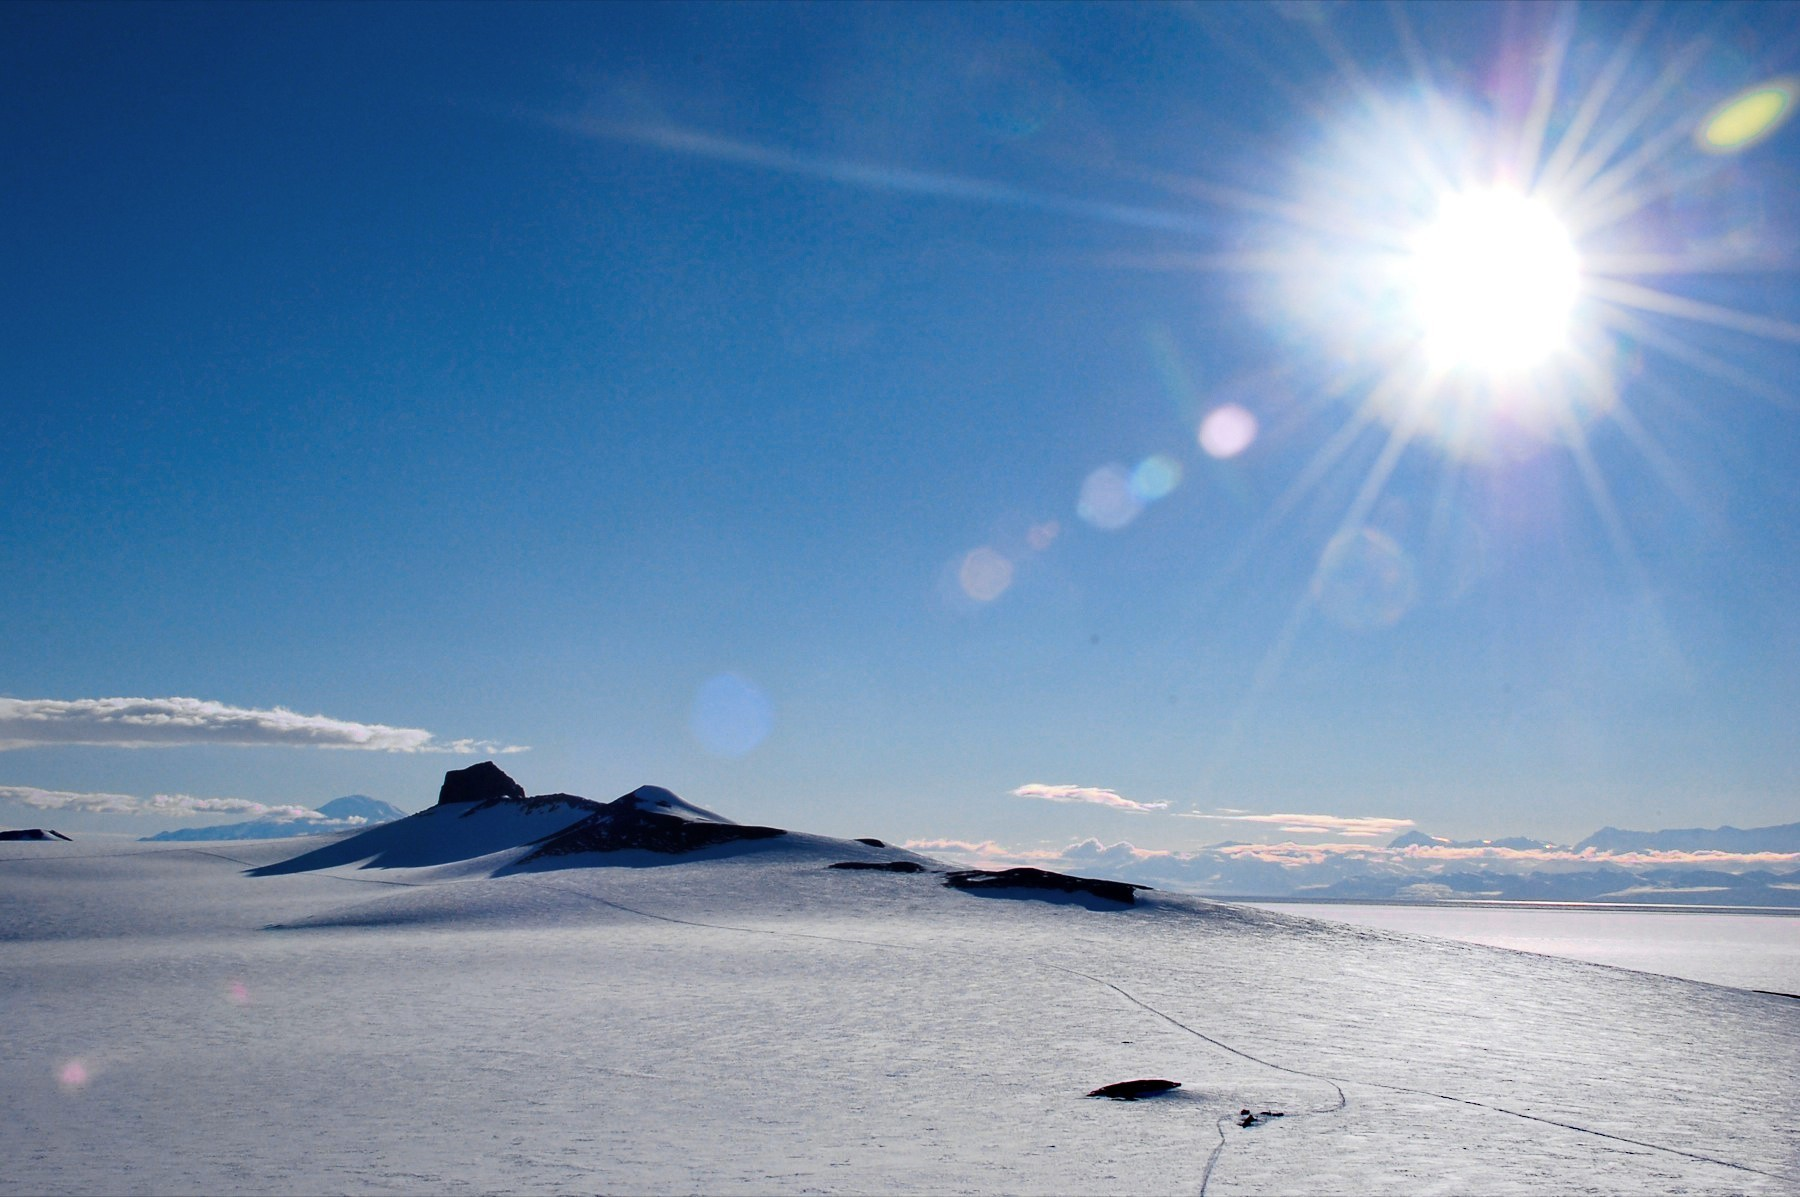
\includegraphics[width=\paperwidth,height=\paperheight]{./images/antarctic_4_tw.jpg}
}

\begin{frame}
  \titlepage
\end{frame}

%%%%%%%%%%%%%%%%%%%%%%%% CLEAR BACKGROUND FOR MAIN SLIDES %%%%%%%%%%%%%%%%%%%%%%

\setbeamertemplate{background}{}
\addtocounter{framenumber}{-1}

%%%%%%%%%%%%%%%%%%%%%%%% MAIN CONTENT %%%%%%%%%%%%%%%%%%%%%%

%% ADD YOUR PRESENTATION HERE - USE A SINGLE WORD TITLE, ALL CAPS



%%%%%%%%%%%%%%%%%%%%%%%% ADD CONTENT %%%%%%%%%%%%%%%%%%%%%%
\section{Intro}
\begin{frame}{\insertsectionnumber{ |} Welcome \& Introduction}

\textbf{Day 1} \\
\vspace*{0.75cm}\begin{tabular}{p{0.75cm}|p{7.5cm}|p{1.75cm}}
\hline 
10:00 & Arrival \& welcome & Nick \\
10:15 & Introduction to programming & Nick \\
& \small{Navigating the command line environment, scripting vs programming, pros \& cons of various languages} & \\
11:30 & Introduction to models & Liz \& Dan \\
& \small{Climate model basics: components, types of models, internal variability. CMIP overview, climate sensitivity} & \\
13:00 & Lunch &  \\
14:00 & Spatial data -- lecture & Alex \& Alena \\
& \small{Understanding gridded data, map projections, data analysis and manipulations, masking, extracting vertical / horizontal sections} & \\
15:30 & Coffee & \\
15:45 & Spatial data -- tutorial & Alex \& Alena \\
17:00 & Wrap-up & \\
\hline
\end{tabular}


\end{frame}

\begin{frame}{\insertsectionnumber{ |} Welcome \& Introduction}

\textbf{Day 2} \\
\vspace*{0.75cm}\begin{tabular}{p{0.75cm}|p{7.5cm}|p{1.75cm}}
\hline\\09:00 & Time-series data -- lecture & Mario \\
& \small{Principal component / empirical orthogonal function analysis, calculation of correlations, anomalies, detrending} & \\
10:30 & Coffee &  \\
10:45 & Time-series data -- tutorial & Mario \\
12:15 & Lunch & \\
13:15 & Document preparation in \LaTeX & Angela \\
& \small{Learn the basics, write equations, insert figures, create your own tables, insert references} & \\
14:45 & Afternoon tea &  \\
15:00 & Work Structure \& Version control & Stefan \\
& \small{Defining a workflow, handling `big data', version control for scripts/documents, best practice guidelines} & \\
\hline
\end{tabular}


\end{frame}

%%%%%%%%%%%%%%%%%%%%%%%%

\begin{frame}{\insertsectionnumber{ |} Aims, Methods, \& Scope}

\begin{columns}

\column[c]{7.5cm}

\begin{itemize}


\begin{beamerboxesrounded}[lower=gray,shadow=true]{\item The \textbf{aim} of the Winter School is that, by the end of the two days, participants will be able to find and download (climate model) data of interest, use simple scripts to process, analyse, and plot those data, integrate these outputs into a typeset document, and use version control software to keep track of changes.}\end{beamerboxesrounded}

\pause\begin{beamerboxesrounded}[lower=gray,shadow=true]{\vspace*{0.5cm}\item We will use \emph{\textbf{Python}} for the majority of the work but will incoporate examples from other languages if necessary. We'll introduce you to packages like \LaTeX ~and tools such as \emph{github}.}\end{beamerboxesrounded}

\pause\begin{beamerboxesrounded}[lower=gray,shadow=true]{\vspace*{0.5cm}\item This workshop is only intended to provide an \textbf{introduction} to working in a command-line environment, and exposure to some of the functionality available in this realm. It is not intended to be a complete course on programming, modelling, or data analysis ;-) }\end{beamerboxesrounded}


\end{itemize}

\end{columns}

\end{frame}


%%%%%%%%%%%%%%%%%%%%%%%% END CONTENT %%%%%%%%%%%%%%%%%%%%%%



%%%%%%%%%%%%%%%%%%%%%%%% ADD CONTENT %%%%%%%%%%%%%%%%%%%%%%
\section{Introduction to programming}
\begin{frame}{\insertsectionnumber{ |} Command-line basics (*nix)}

\hspace*{-0.5cm}\textbf{Basic commands} \\
\vspace*{0.25cm}\begin{tabular}{p{0.75cm} p{6cm} p{3.5cm}}
\textbf{command} & \textbf{~~example} & \textbf{description} \\
ls & \Verb+ ls -ltrh + & \ul{l}i\ul{s}t directory contents (in long format, newest last) \\
cd & \Verb+ cd ../mydir/mysubdir + & \ul{c}hange \ul{d}irectory (up one level, down two) \\
rm & \Verb+ rm delete-this.txt and-all-these.* + & \ul{r}e\ul{m}ove file(s) \\
mv & \Verb+ mv rename-this.txt to-this.txt + & \ul{m}o\ul{v}e (rename) file(s) \\
mkdir & \Verb+ mkdir ./new-directory + & \ul{m}a\ul{k}e a new (empty) \ul{dir}ectory  \\
cp & \Verb+ cp this.txt ./new-dir/to-this.txt + & \ul{c}o\ul{p}y file (possibly to new location) \\
\end{tabular}


\vspace*{0.5cm}\hspace*{-0.5cm}\textbf{Linux c-line tools} \\
\begin{tabular}{p{0.75cm} p{6cm} p{3.5cm}}
\textbf{tool} & \textbf{~~example} & \textbf{description} \\
pwd & \Verb+ pwd + & Find out what your current \ul{p}ersonal \ul{w}orking \ul{d}irectory is \\
sed & \Verb+ sed -e 's/a/b/g'+ & \ul{s}tream \ul{ed}itor, swap `a' for `b' \\
awk & \Verb+ awk '\{print \$2, \$3\}'+ & print fields 2 \& 3 from file/stream \\
\end{tabular}

\vspace*{0.5cm}\hspace*{-0.5cm}\textbf{Other packages \& utilities} \\
\begin{tabular}{p{0.75cm} p{6cm} p{3.5cm}}
\textbf{package} & \textbf{~~example} & \textbf{description} \\
pdflatex & \Verb+ pdflatex myfile.tex + & compile \LaTeX document \\
git & \Verb+ git clone golledni/WinterSchool + & Make a local copy of a github repository \\
\end{tabular}


\end{frame}

%%%%%%%%%%%%%%%%%%%%%%%%

%\begin{frame}{\insertsectionnumber{ |} Aims, Methods, \& Scope}
%
%\begin{columns}
%
%\column[c]{7.5cm}
%
%\begin{itemize}
%
%
%\begin{beamerboxesrounded}[lower=gray,shadow=true]{\item }\end{beamerboxesrounded}
%
%\begin{beamerboxesrounded}[lower=gray,shadow=true]{\vspace*{0.5cm}\item }\end{beamerboxesrounded}
%
%\begin{beamerboxesrounded}[lower=gray,shadow=true]{\vspace*{0.5cm}\item }\end{beamerboxesrounded}
%
%
%\end{itemize}
%
%\end{columns}
%
%\end{frame}


%%%%%%%%%%%%%%%%%%%%%%%% END CONTENT %%%%%%%%%%%%%%%%%%%%%%

\section{Climate modelling}
%\nopagecolor
%\includepdf[pages=1]{climate-model-lecture.pdf}
%%%%%%%%%%%%%%%%%%%%%%%% ADD CONTENT %%%%%%%%%%%%%%%%%%%%%%

\section{Analysis and plotting of spatial data}
\begin{frame}
   \vspace{1cm}
    \Huge{
   FROM FILE  .....   \\
   \vspace{0.5cm}
   \hspace{5cm}  TO FIGURE ...  \\}
   
\includegraphics[scale=0.5]{images/penguin-graph-cover.png}
\end{frame}

%*****************************************************************
% SEC0 | Outline
%*****************************************************************

\begin{frame}{\insertsectionnumber{ |} Outline}
   \begin{itemize}
       \item Downloaded a file, so what?
            \vspace{0.3cm}
       \item Play around with CDO
            \vspace{0.3cm}
       \item Load into Python and visualise
            \vspace{0.3cm}
       \item Make a publication figure
   \end{itemize}
\end{frame}

%*****************************************************************
% SEC1 | Downloaded a file, so what?
%*****************************************************************
\begin{frame}{\insertsectionnumber{ |} Downloaded a file, so what?}
\end{frame}

\begin{frame}{\insertsectionnumber{ |} Downloaded a file, so what? - Using \textbf{ncview}}
   \begin{itemize}
       \item What are the dimensions? what is the domain?
            \vspace{0.3cm}
       \item What are the variables?
            \vspace{0.3cm}
       \item What are the units? and range?
            \vspace{0.3cm}
       \item Is there masked data? what is the value used? 
            \vspace{0.3cm}
       \item How to create a quick timeseries?
   \end{itemize}
\end{frame}


\begin{frame}{\insertsectionnumber{ |} Downloaded a file, so what? - Using \textbf{ncview}}
    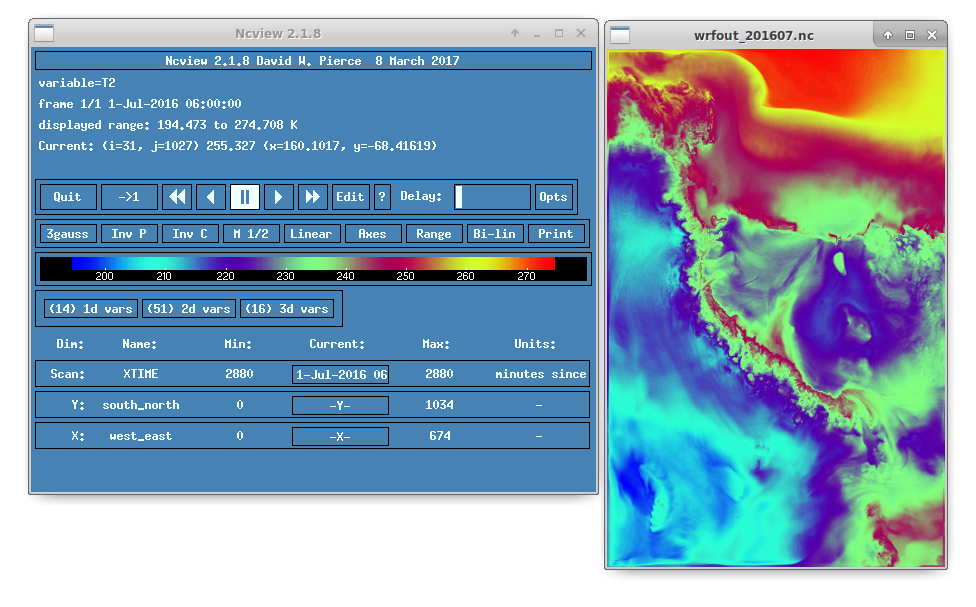
\includegraphics[scale=0.35]{images/wrf_RIS.png}\\
        \centering{WRF output, 2m temperature}
\end{frame}


% \begin{frame}{\insertsectionnumber{ |} Downloaded a file, so what? - Using \textbf{ncview}}
%     Using \textbf{ncview} to check the file:
%     \begin{columns}
%         \column[c]{6.5cm}
%             \centering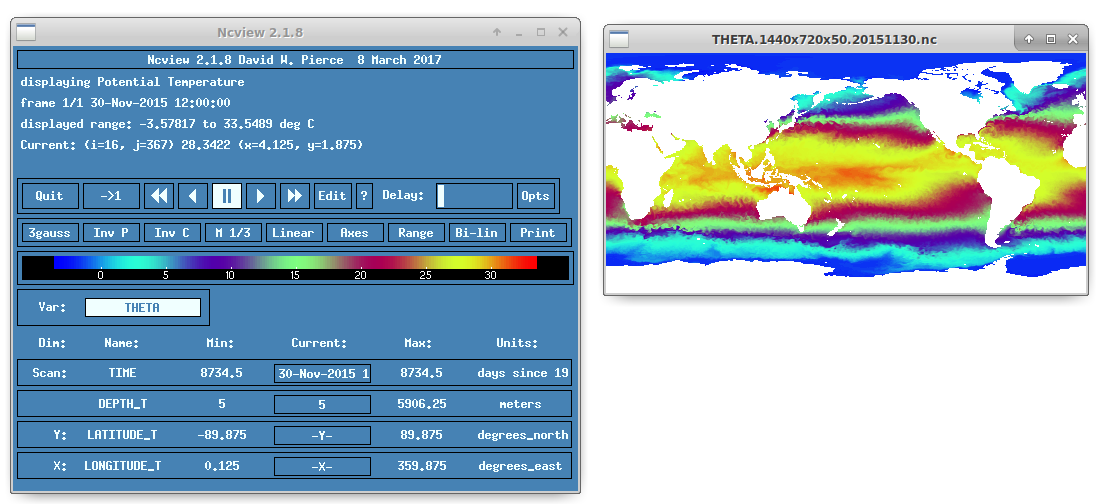
\includegraphics[width=6cm]{images/Theta.png} \\
%                 \centering{ECCO2, potential temperature}
%         \column[c]{6.5cm}
%     \end{columns}
% \end{frame}


\begin{frame}{\insertsectionnumber{ |} Downloaded a file, so what? - Using \textbf{ncview}}
    \begin{columns}
        \column[c]{6.5cm}
            \centering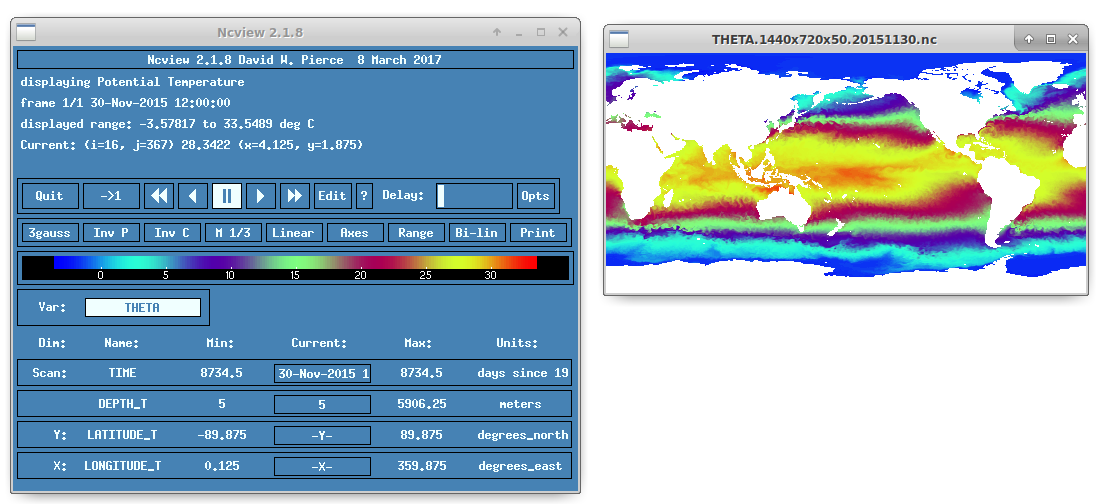
\includegraphics[width=6cm]{images/Theta.png} \\
                \centering{ECCO2, potential temperature}
        \column[c]{6.5cm}
            \centering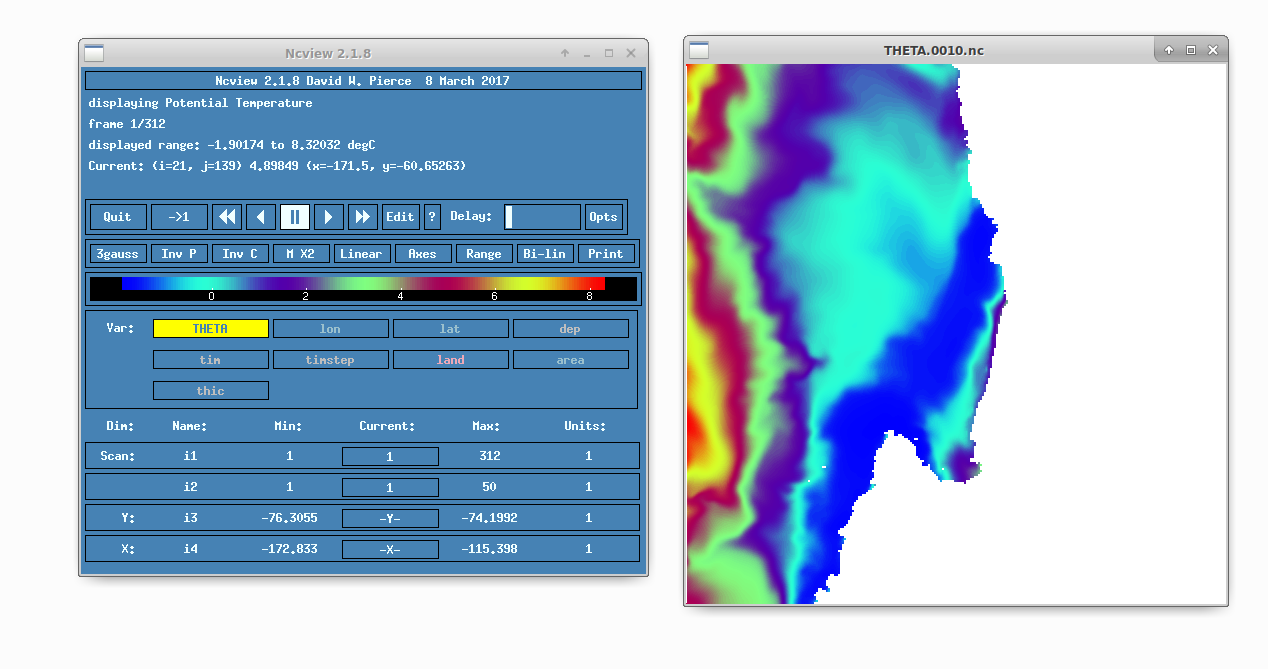
\includegraphics[width=6cm]{images/MIT_eccoV5.png} \\
                \centering{ECCO v5, potential temperature}
    \end{columns}
\end{frame}


\begin{frame}{\insertsectionnumber{ |} Downloaded a file, so what? - Using \textbf{ncview}}
    \flushleft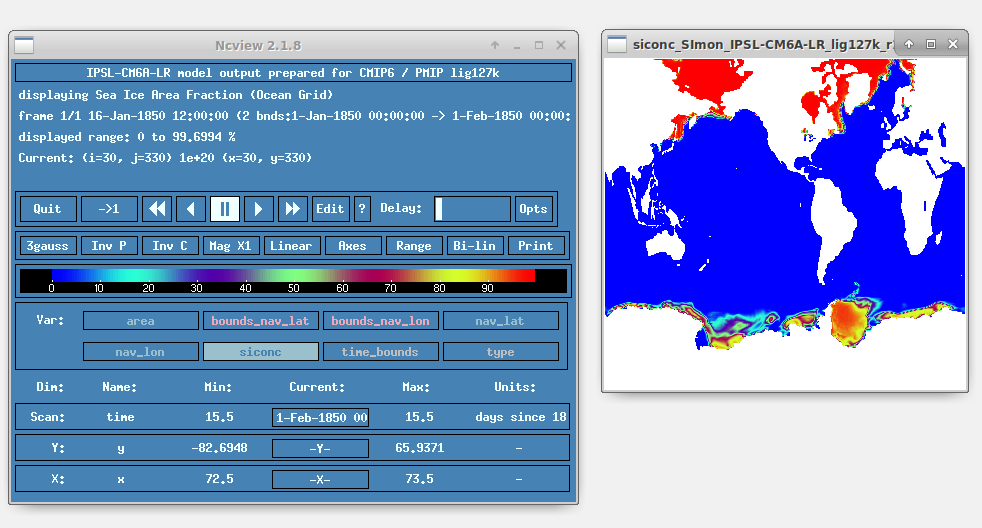
\includegraphics[scale=0.33]{images/tripolar.png}\hspace*{1cm}\\
        \centering{IPSL-CM6A-LR, sea ice area fraction}
\end{frame}


\begin{frame}{\insertsectionnumber{ |} Downloaded a file, so what? - Using \textbf{panoply}}
    \centering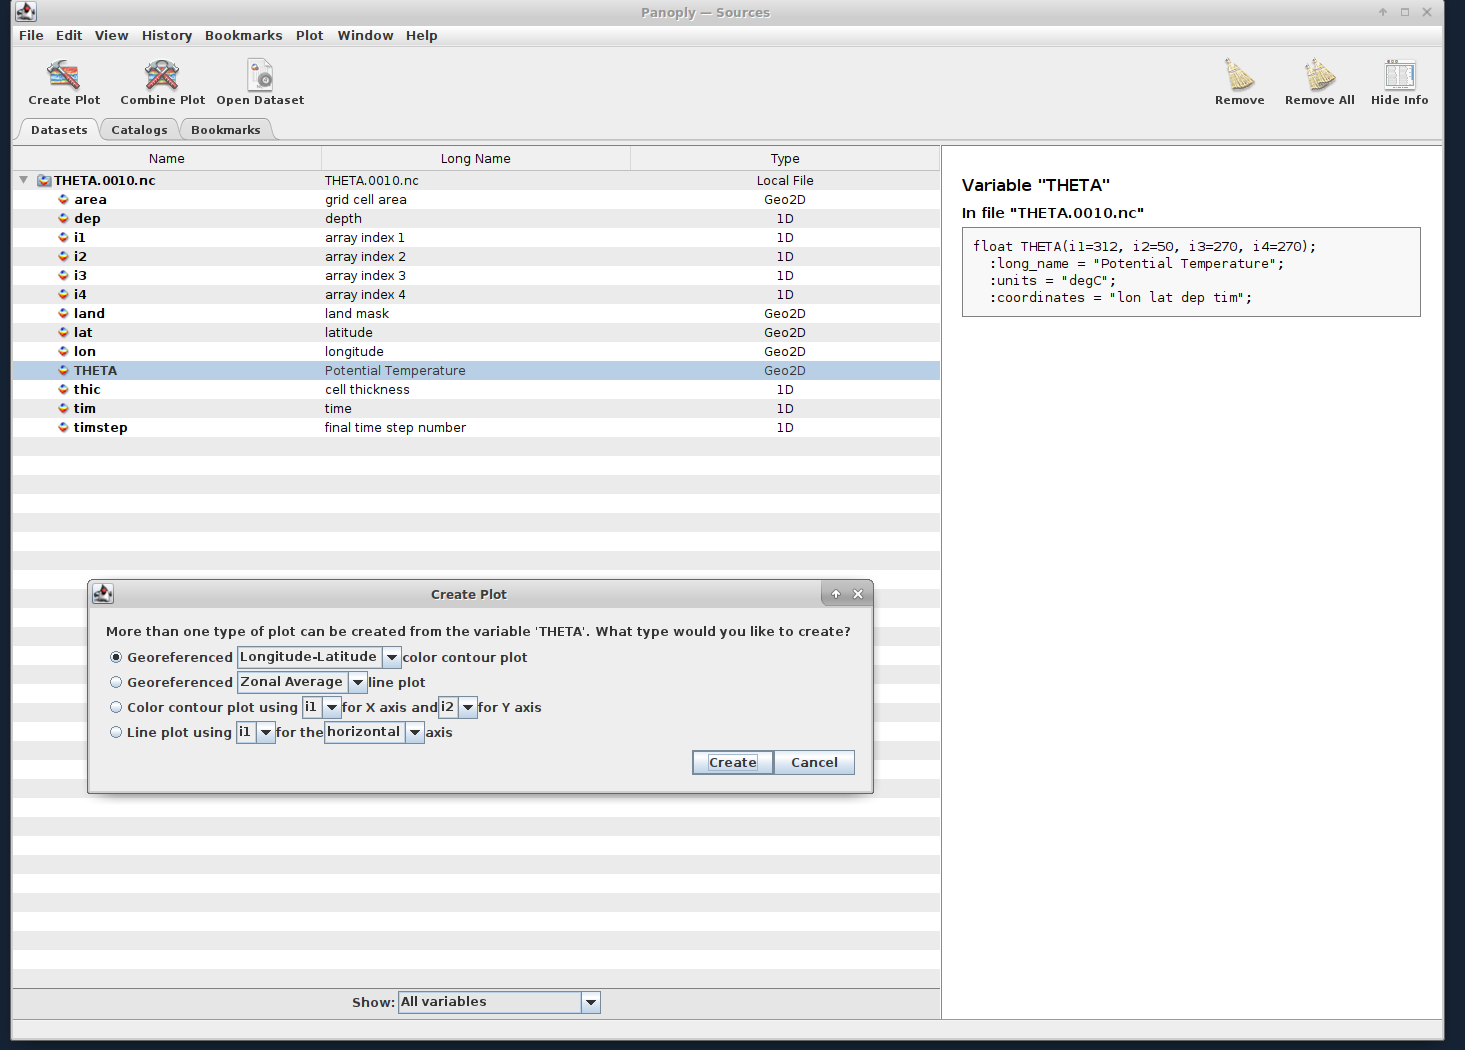
\includegraphics[width=10cm]{images/Panoply1.png} \\
\end{frame}


\begin{frame}{\insertsectionnumber{ |} Downloaded a file, so what? - Using \textbf{panoply}}
    \centering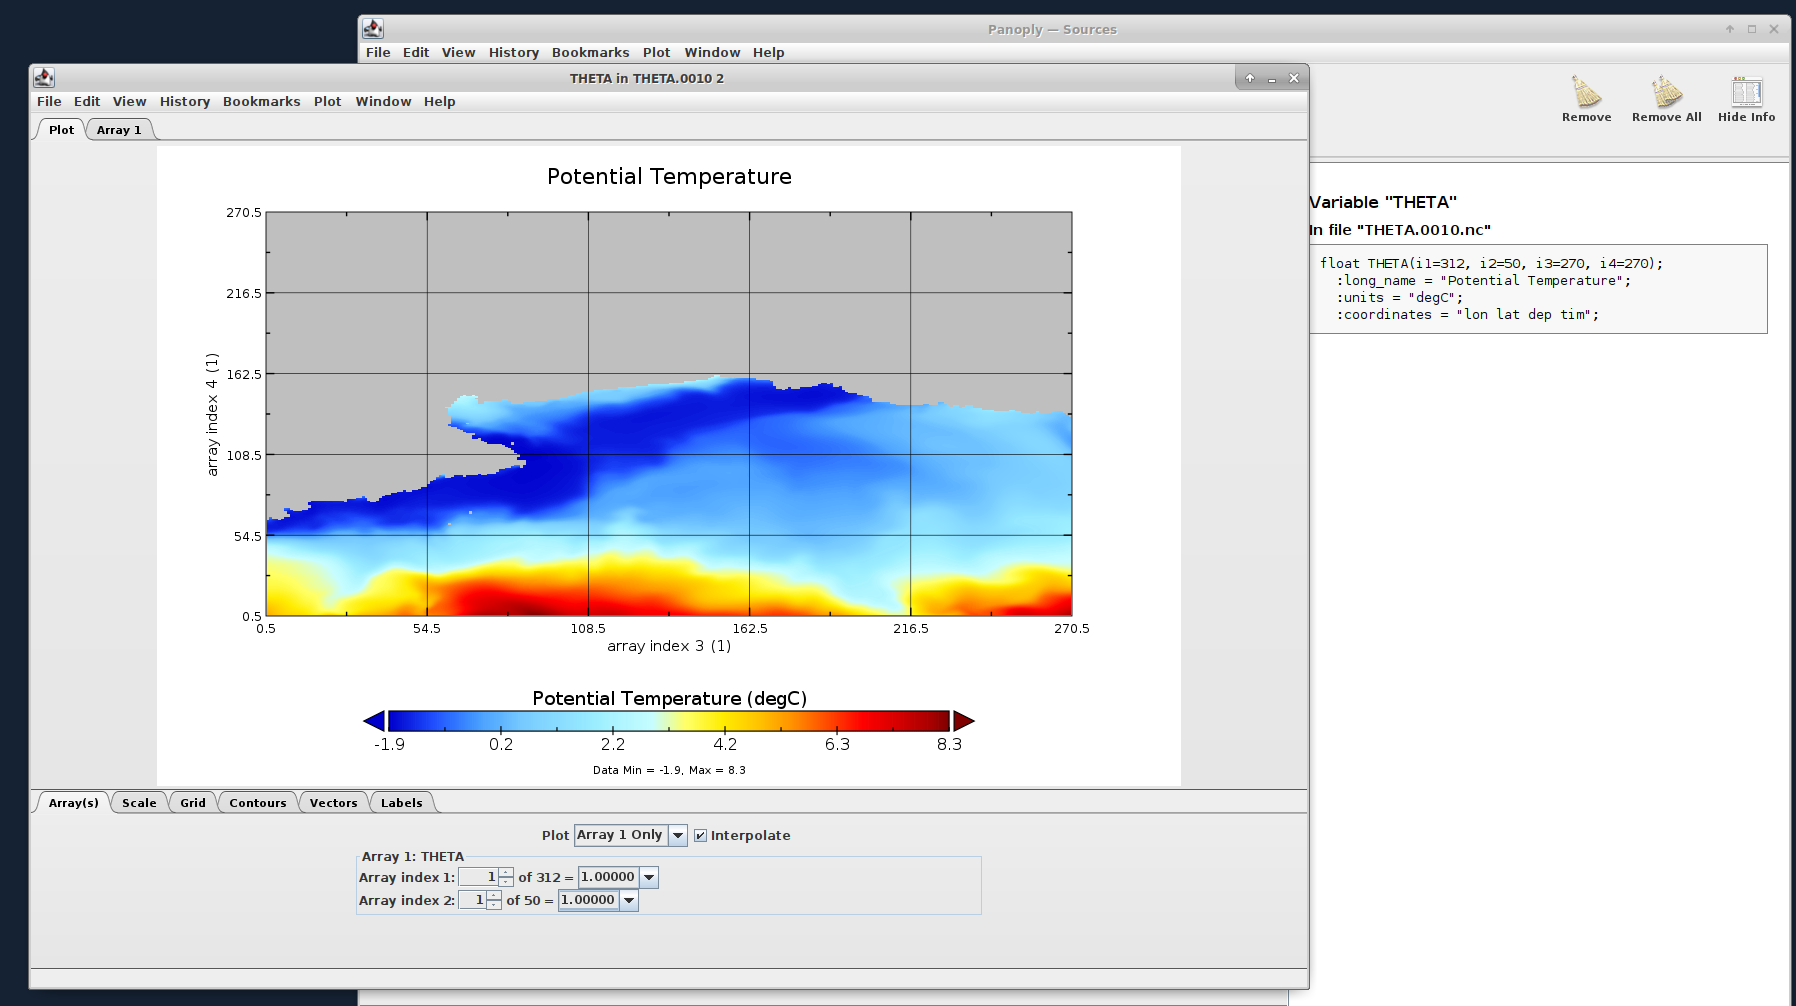
\includegraphics[width=10cm]{images/Panoply2.png} \\
\end{frame}


\begin{frame}{\insertsectionnumber{ |} Downloaded a file, so what? - Using \textbf{panoply}}
    \centering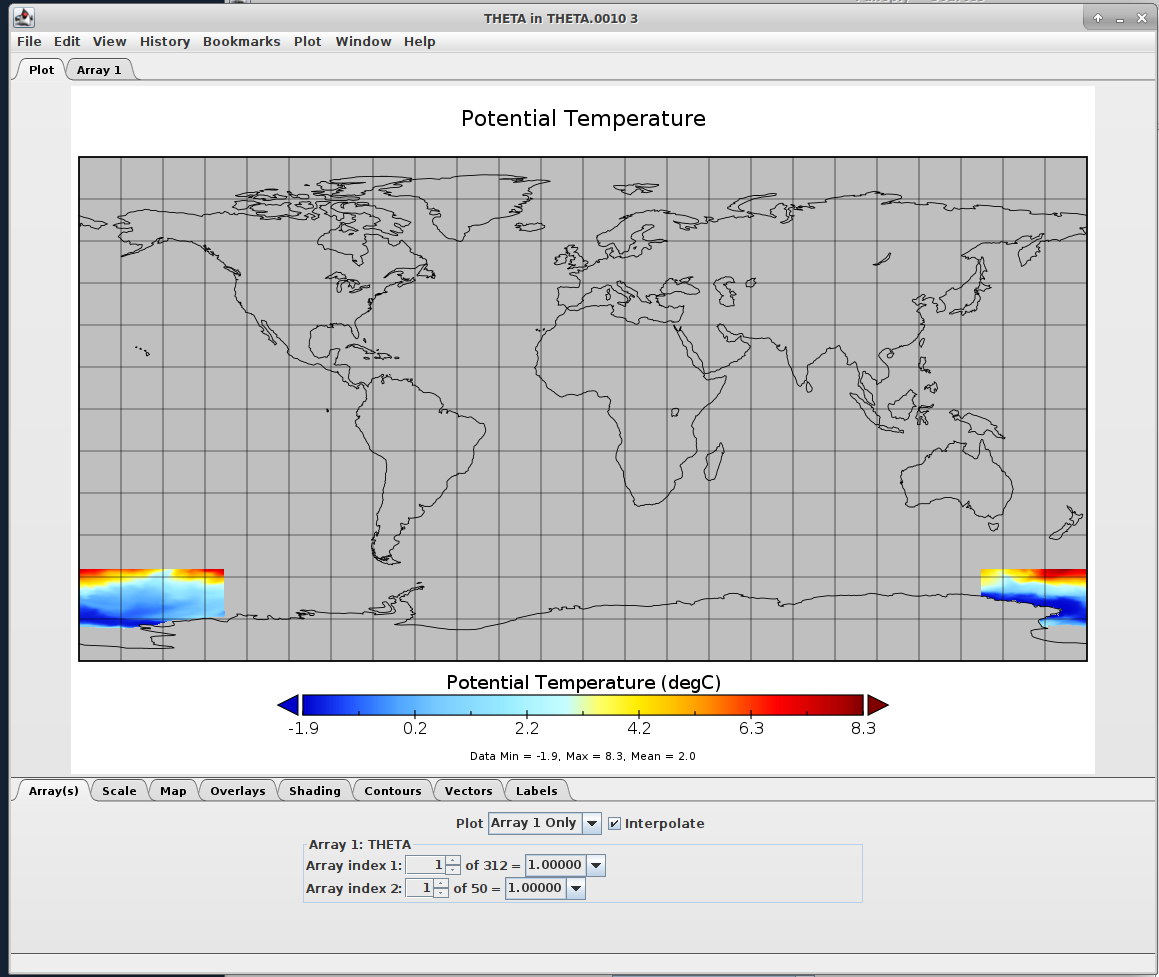
\includegraphics[width=8.5cm]{images/Panoply3.png} \\
\end{frame}


\begin{frame}{\insertsectionnumber{ |} Downloaded a file, so what? - Using \textbf{panoply}}
    \centering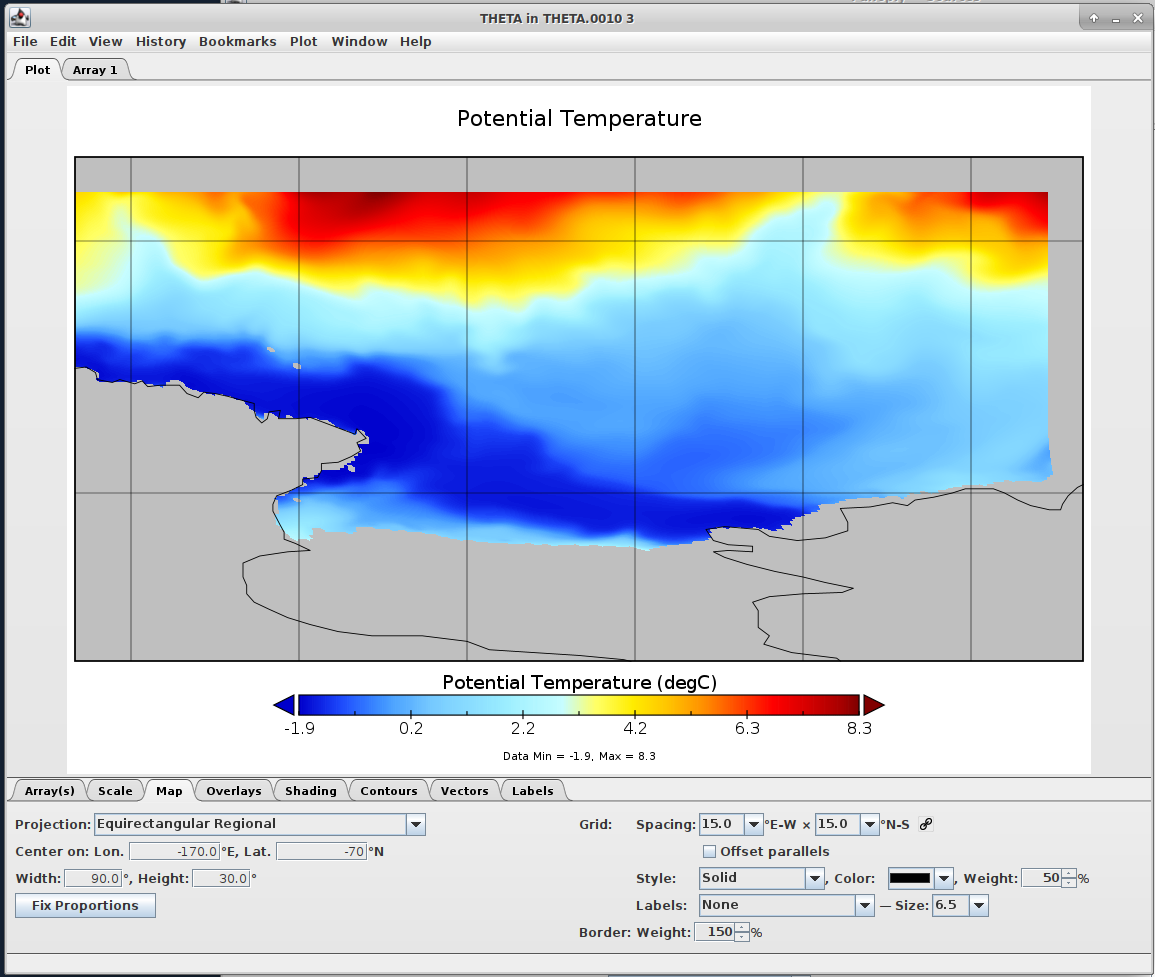
\includegraphics[width=8.5cm]{images/Panoply4.png} \\
\end{frame}


\begin{frame}{\insertsectionnumber{ |} Downloaded a file, so what? - Using \textbf{panoply}}
    \centering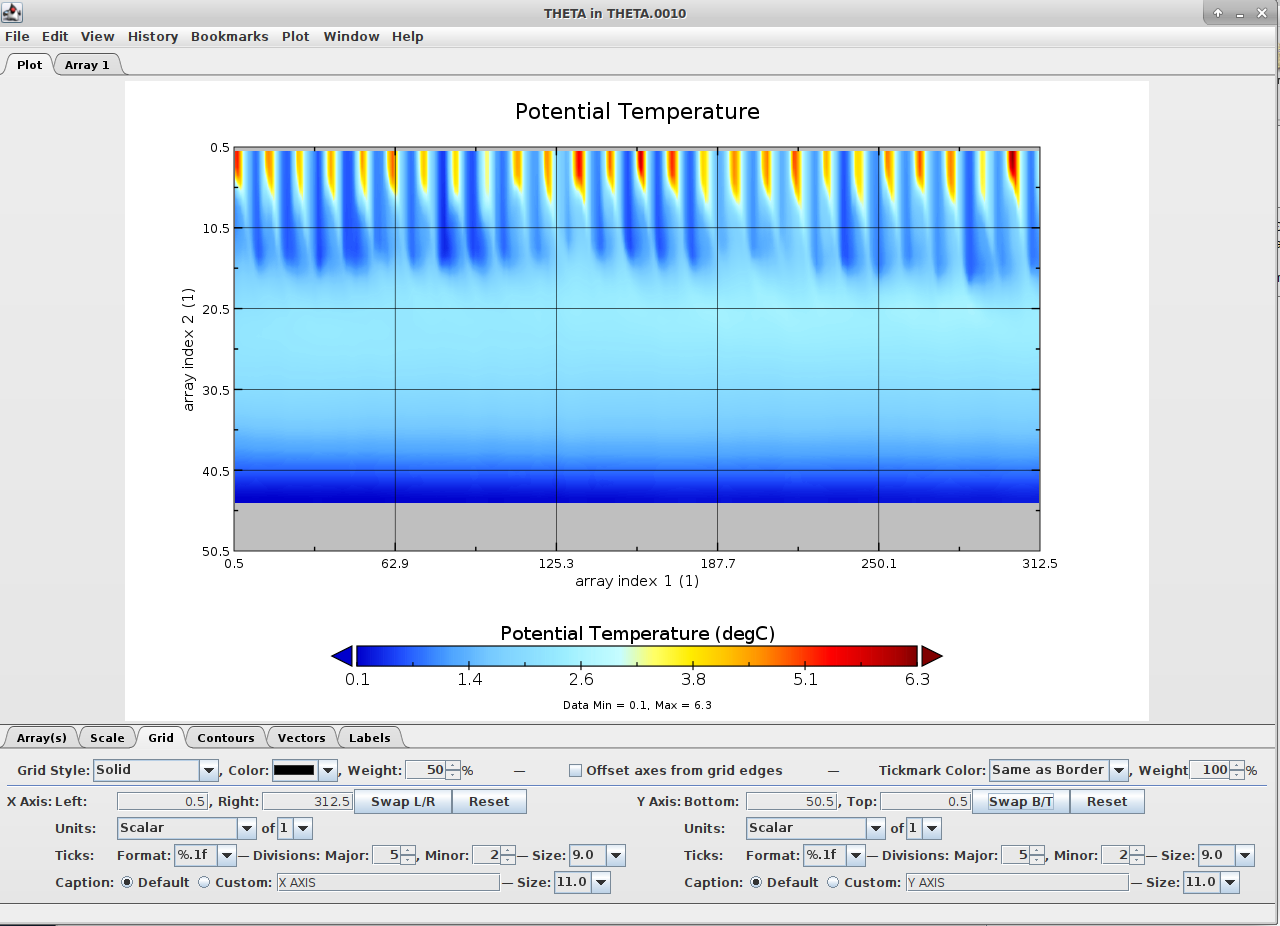
\includegraphics[width=10cm]{images/Panoply5.png} \\
\end{frame}


\begin{frame}{\insertsectionnumber{ |} Downloaded a file, so what? - Using \textbf{panoply}}
    \centering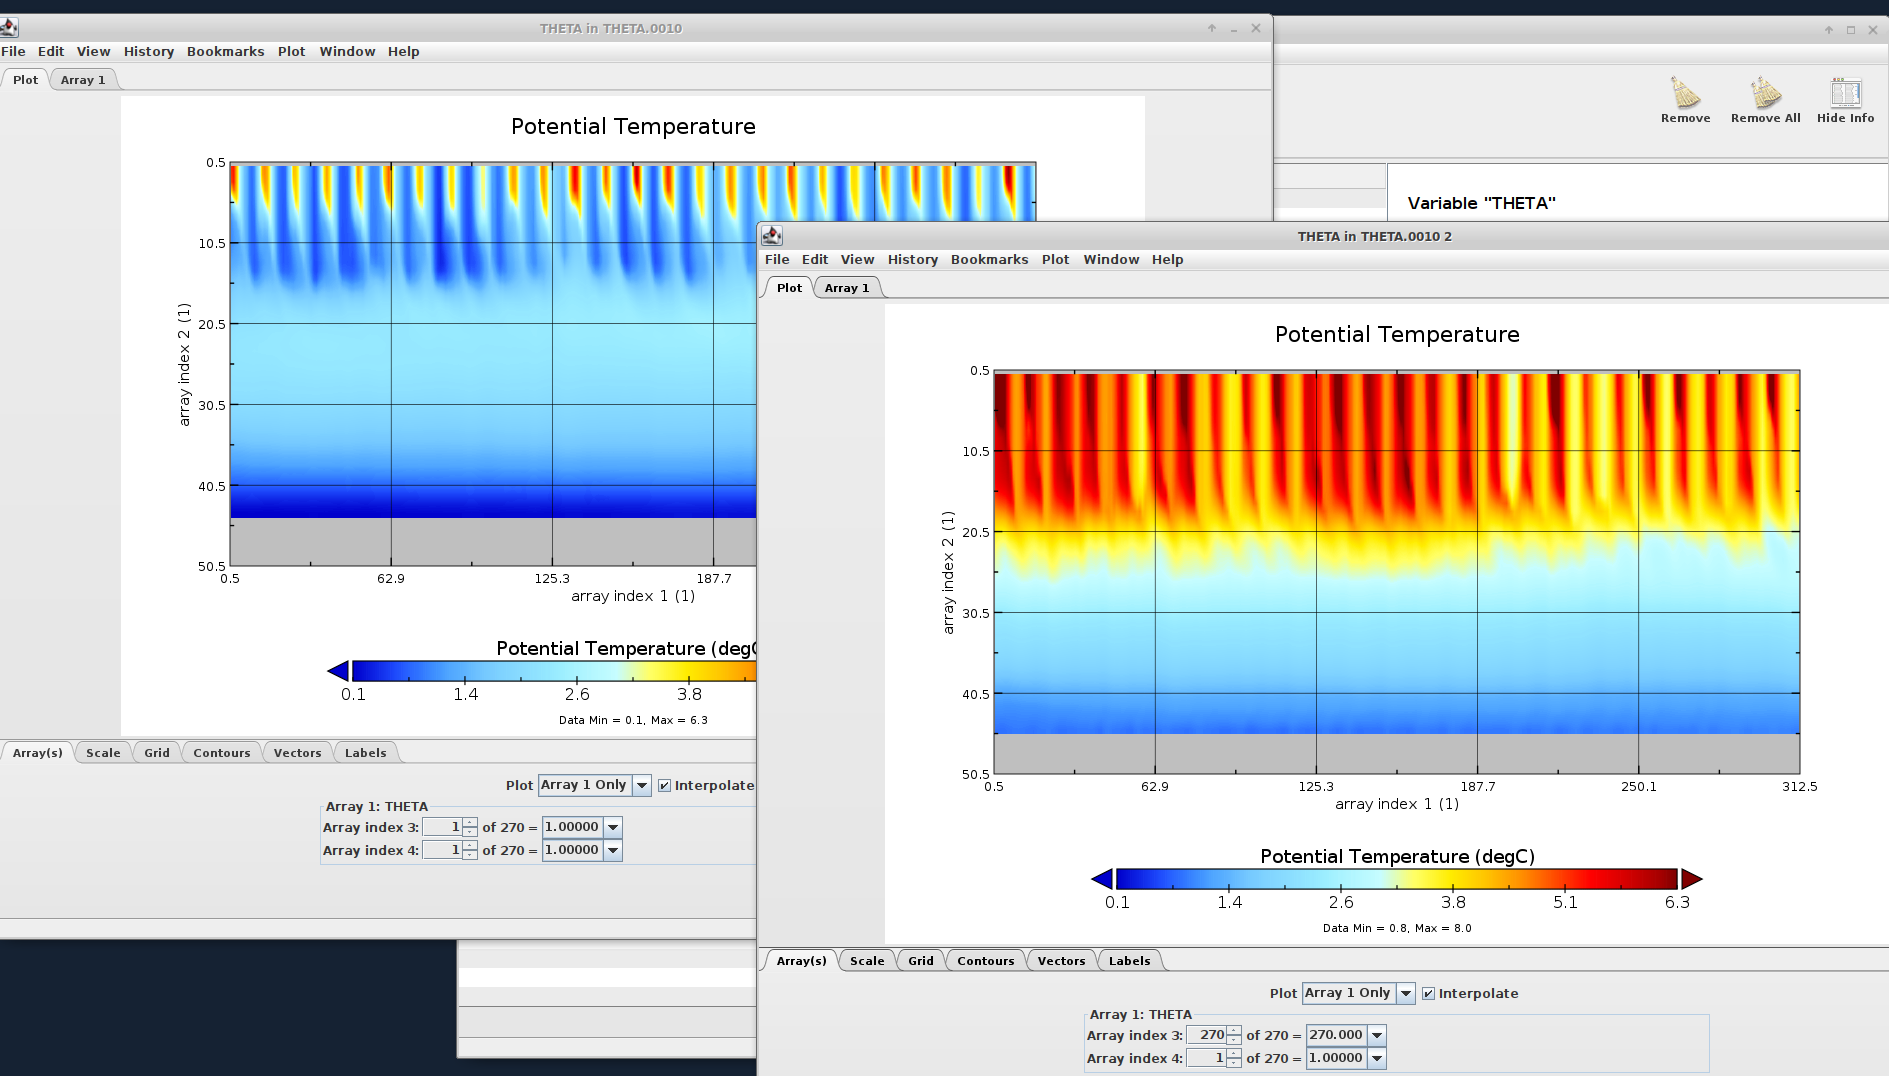
\includegraphics[width=10cm]{images/Panoply6.png} \\
\end{frame}


\begin{frame}{\insertsectionnumber{ |} Downloaded a file, so what? - Using \textbf{panoply}}
    \centering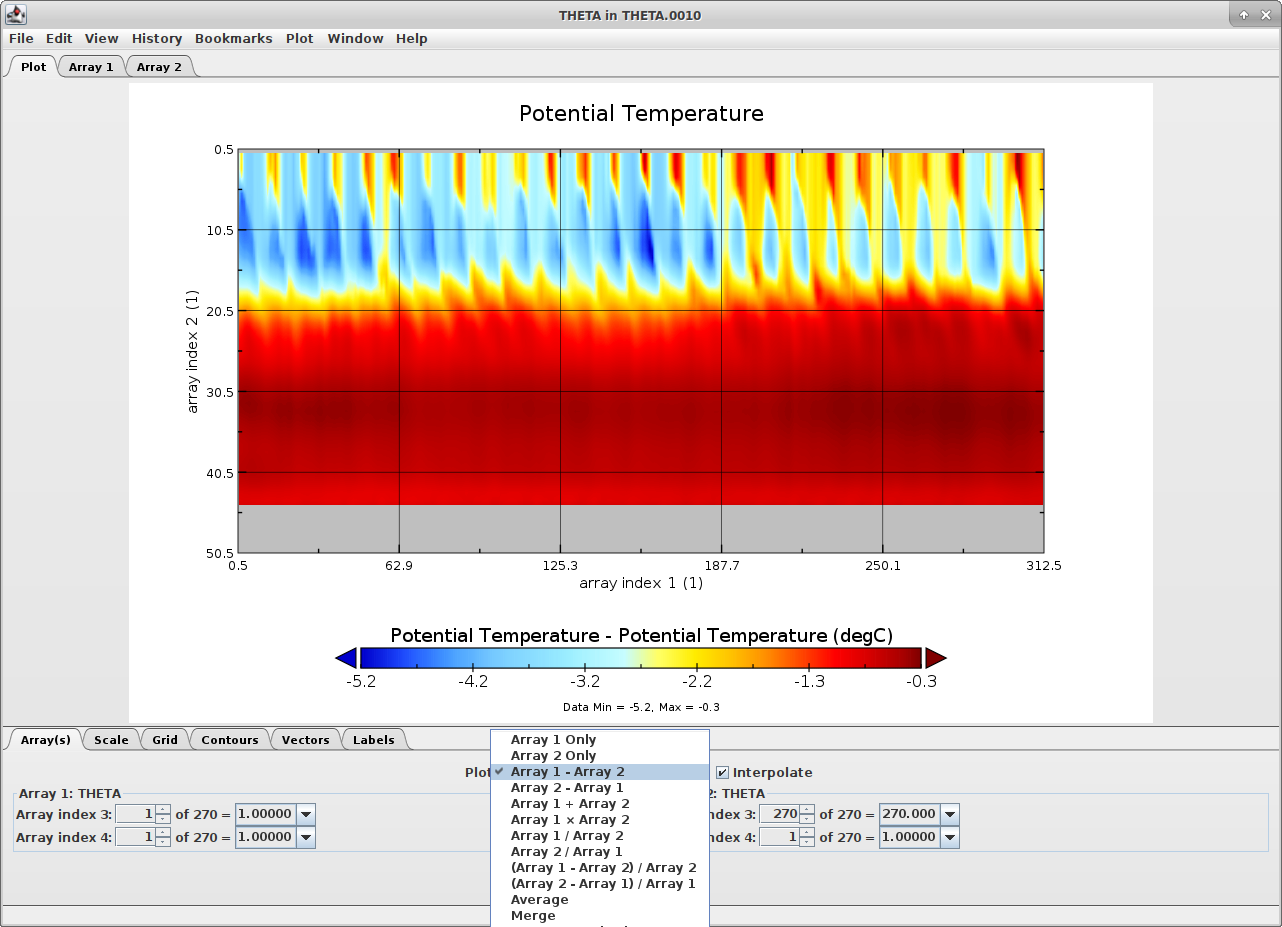
\includegraphics[width=10cm]{images/Panoply7.png} \\
\end{frame}


\begin{frame}{\insertsectionnumber{ |} Downloaded a file, so what? - Using \textbf{panoply}}
    \centering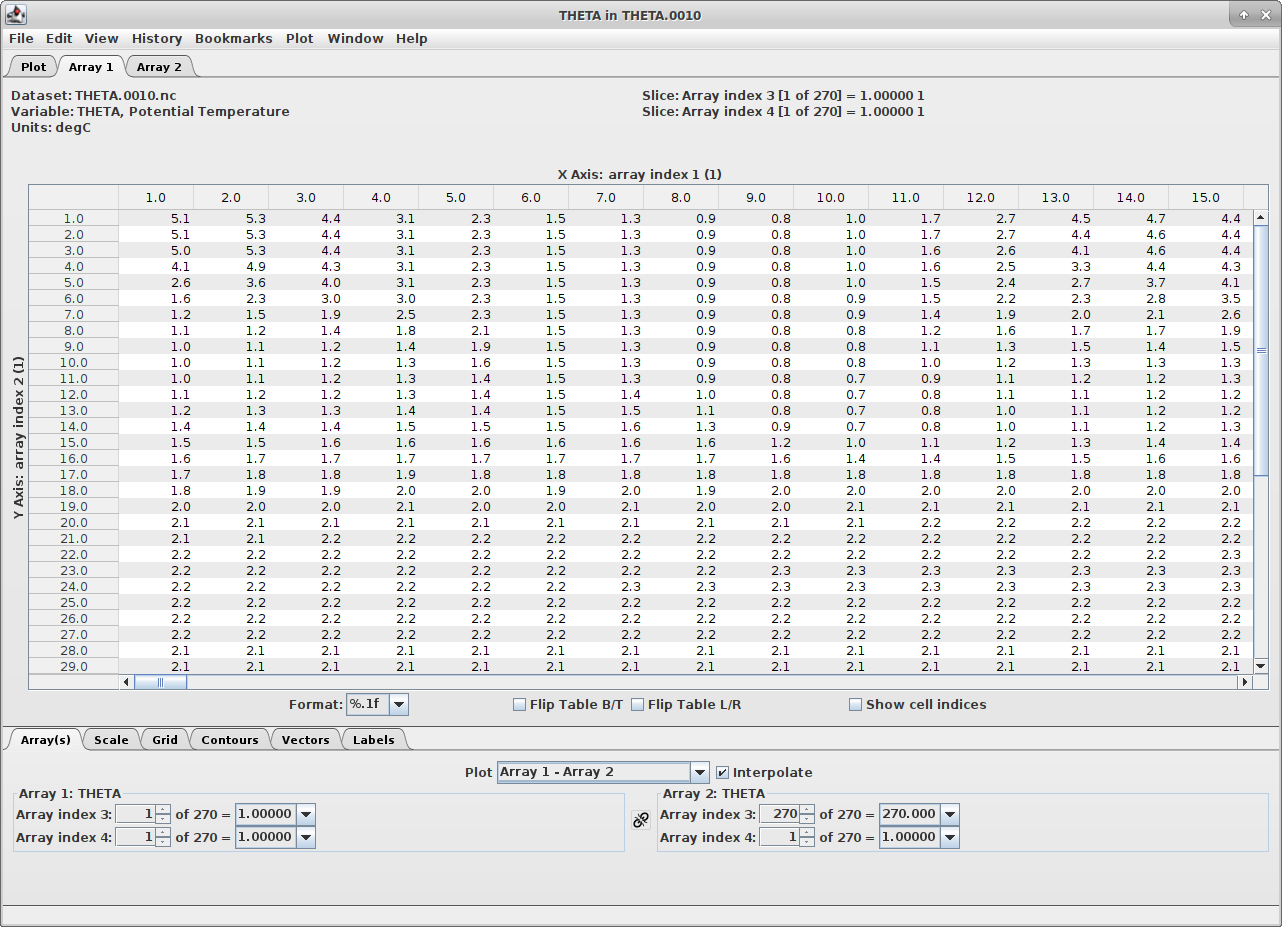
\includegraphics[width=10cm]{images/Panoply8.png} \\
\end{frame}


\begin{frame}{\insertsectionnumber{ |} Downloaded a file, so what? - \textbf{coordinates}}
    Different coordinate systems:
        \vspace{0.3cm}
    \begin{itemize}
        \item lon-lat (easy to figure out where we are)
            \vspace{0.3cm}
        \item x-y (equidistant grid in km, better at the poles)
            \vspace{0.3cm}
        \item irregular grid (removes the pole problem)
    \end{itemize}
\end{frame}


\begin{frame}{\insertsectionnumber{ |} Downloaded a file, so what? - \textbf{coordinates}}
    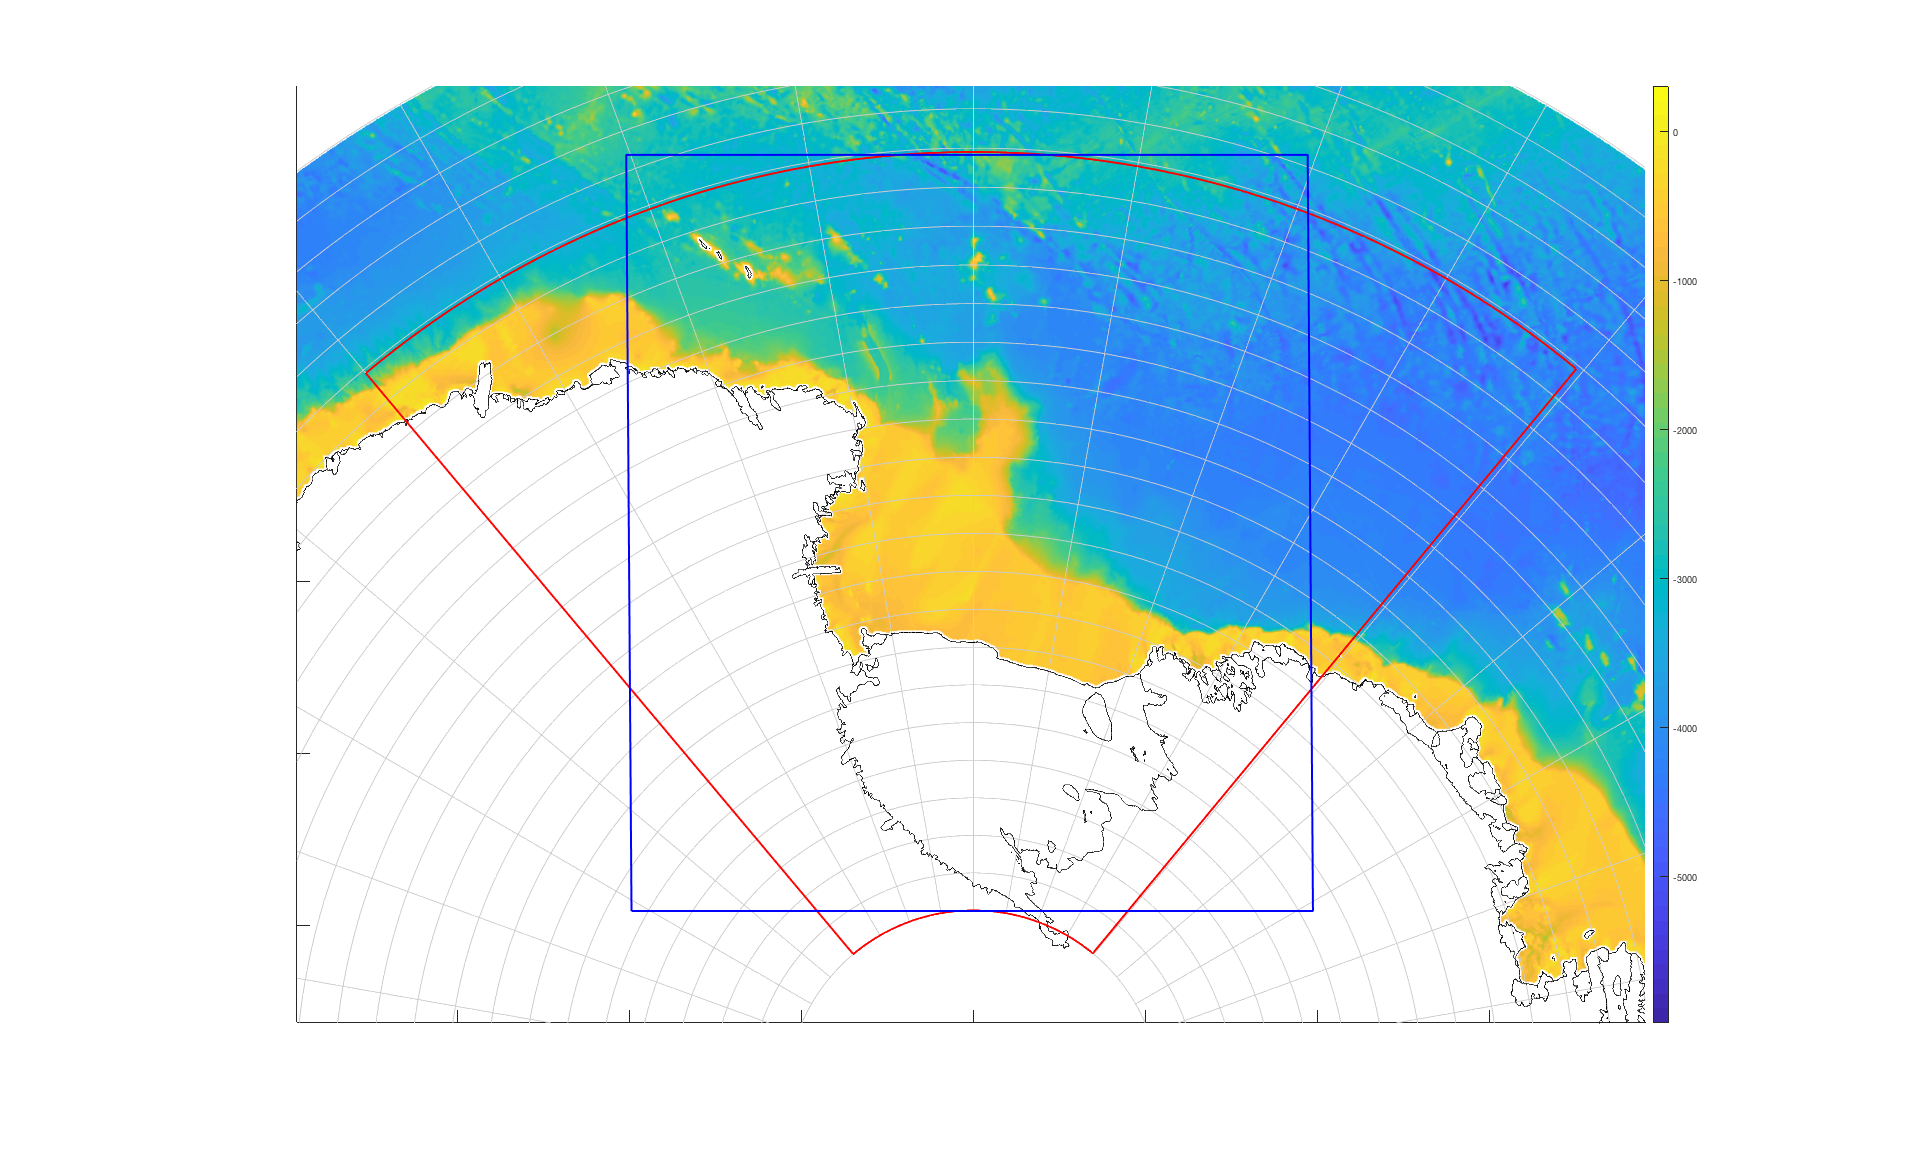
\includegraphics[scale=0.25]{images/winter_school_domain_1.png}
\end{frame}


\begin{frame}{\insertsectionnumber{ |} Downloaded a file, so what? - \textbf{coordinates}}
    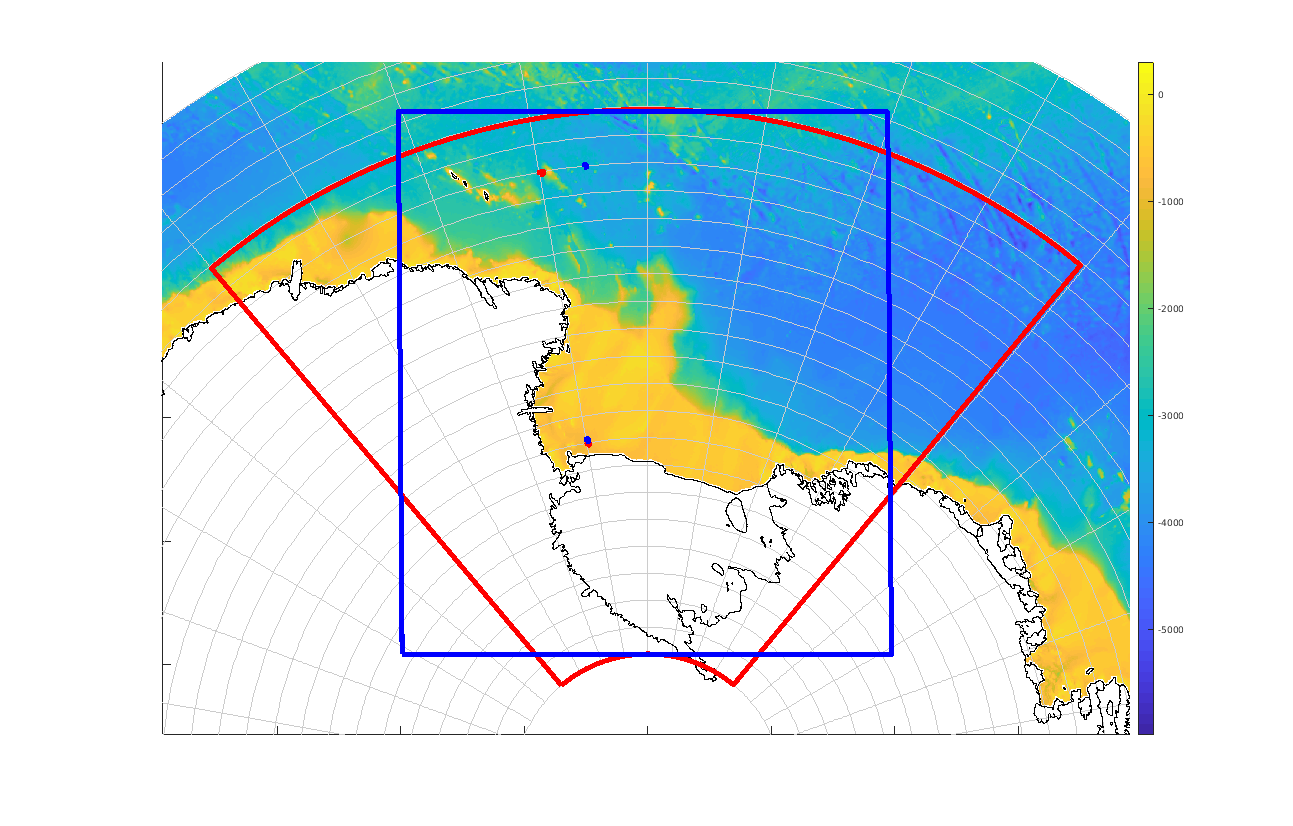
\includegraphics[scale=0.25]{images/winter_school_domain_2.png}
\end{frame}


\begin{frame}{\insertsectionnumber{ |} Downloaded a file, so what? - \textbf{coordinates}}
    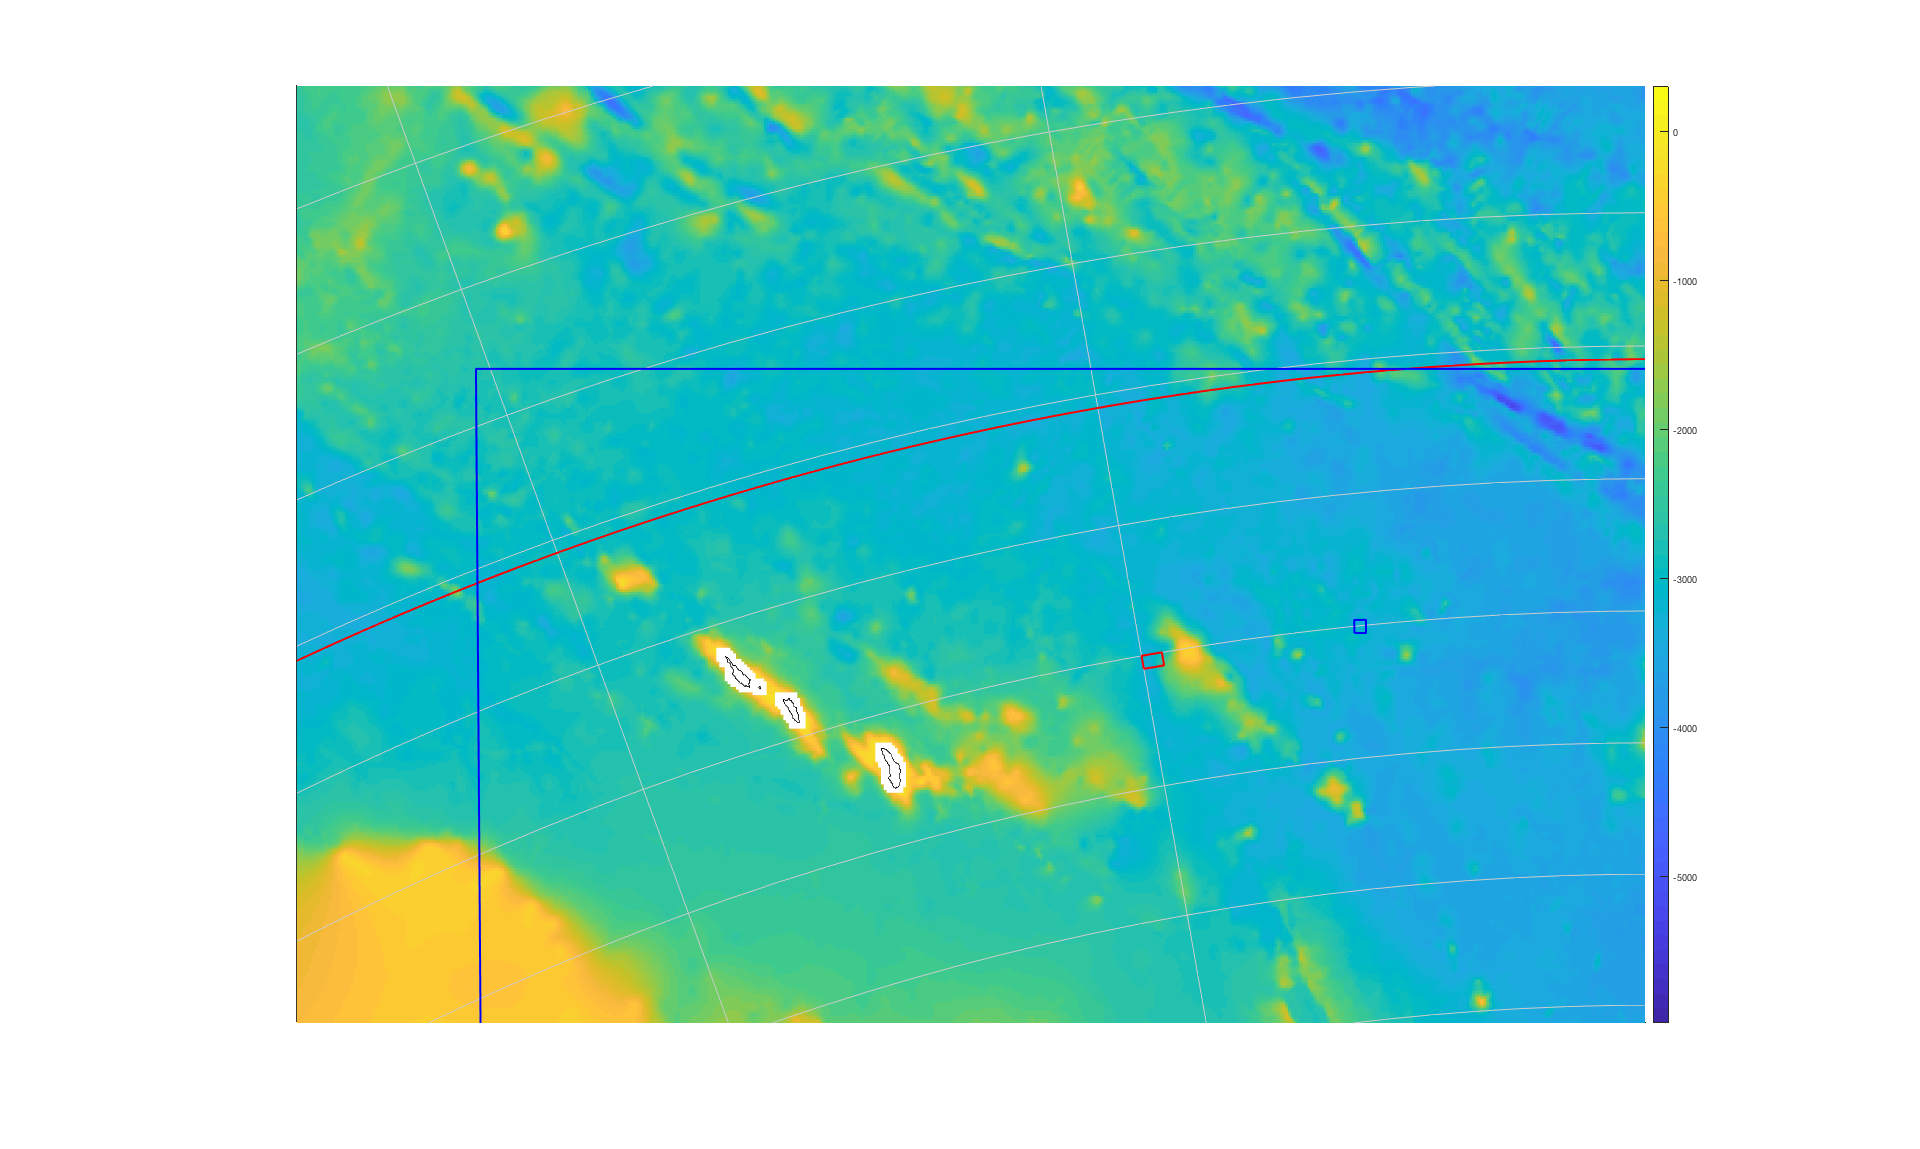
\includegraphics[scale=0.25]{images/winter_school_domain_3.png}
\end{frame}

\begin{frame}{\insertsectionnumber{ |} Downloaded a file, so what? - \textbf{coordinates}}
    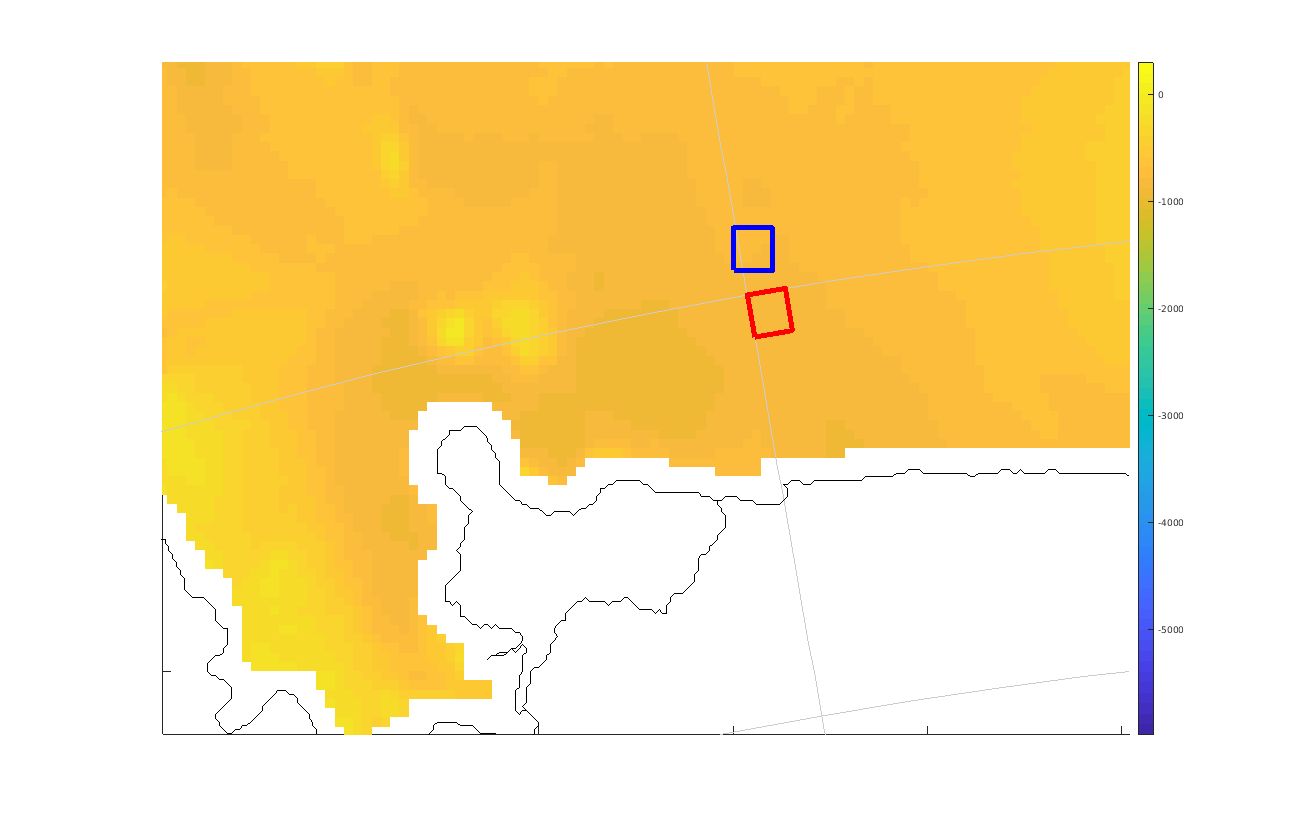
\includegraphics[scale=0.25]{images/winter_school_domain_3_2.png}
\end{frame}

\begin{frame}{\insertsectionnumber{ |} Downloaded a file, so what? - get information on the data}
    \begin{itemize}
        \item The naming \textbf{conventions} are useful: what do the two files contain?\\
            \vspace{0.5cm}
        \item Let's verify using \textbf{ncview} or \textbf{cdo}: \\
            \begin{itemize}
                \item \textit{ncdump filename} 
                \item \textit{ncdump -h filename} 
                \item \textit{cdo sinfo filename} 
            \end{itemize}
        \vspace{2cm}
    \begin{beamerboxesrounded}[lower=gray,shadow=true]{Pop quiz: open the theta....2013.nc file and:
        \begin{itemize}
            \item what is the variable(s)? short and long name?
            \item what is the spatial resolution of the data? and the dimension of the file?
            \item what is the temporal coverage of the data?
         \item is there a mask value anywhere? 
         \item how many dimensions does this variable have?
        \end{itemize}
        }
    \end{beamerboxesrounded}
    \end{itemize}
\end{frame}
 
 
%*****************************************************************
% SEC2 | Play around with CDO
%*****************************************************************
\begin{frame}{\insertsectionnumber{ |} Play around with \textbf{cdo}}
\end{frame} 


\begin{frame}{\insertsectionnumber{ |} Play around with \textbf{cdo}}
    Manipulating big files can be slow or make your program crash!\\
        \vspace{0.3cm}
    Pre-processing can save our life: let's use \href{http://www.idris.fr/media/ada/cdo.pdf}{\beamerbutton{\Huge{CDO}}}\\
        \vspace{0.5cm}
    \textbf{cdo} can be used to :
        \vspace{0.3cm}
    \begin{itemize}
        \item select
            \vspace{0.1cm}
            \begin{itemize}
                \item spatially
                    \vspace{0.1cm}
                \item temporally
                    \vspace{0.1cm}
                \item vertically
            \end{itemize}
        \item mask
        \item remap
        \item do statistics and calculations
        \item and so much more...
    \end{itemize}
\end{frame}     
        
\begin{frame}{\insertsectionnumber{ |} Play around with \textbf{cdo} - spatial extent}        
    To reduce the \textbf{spatial} extent:
    \vspace{0.3cm}
    \begin{itemize}
        \item \textit{cdo sellonlatbox,lon0,lon1,lat0,lat1 infile outfile }
           \vspace{0.3cm}
        \item \textit{cdo selindexbox,index0,index1,index0,index1 infile outfile }
    \end{itemize}
        \vspace{0.5cm}
    example: to select New Zealand (to be done on both theta and so files)\\
        \vspace{0.3cm}
    \textcolor{black}{cdo sellonlatbox,150,180,-30,-50 thetao\_Omon\_CESM2\_historical\_r1i1p1f1\_gr\_201301-201412.nc NZ\_theta.nc }\\
        \vspace{0.3cm}
\end{frame}
  
  
\begin{frame}{\insertsectionnumber{ |} Play around with \textbf{cdo} - temporal extent}
    To reduce the \textbf{temporal} extent:
        \vspace{0.3cm}
    \begin{itemize} 
        \item \textit{cdo selmon,1 infile outfile }
            \vspace{0.3cm}
        \item \textit{cdo select,timestep=1  infile outfile }
            \vspace{0.3cm}
         \item \textit{cdo splityear  infile prefix- }
    \end{itemize}
\end{frame}


\begin{frame}{\insertsectionnumber{ |} Play around with \textbf{cdo} - vertical (level) extent}
    To reduce the number of \textbf{levels}:\\
        \vspace{0.3cm}
    \begin{itemize}
        \item \textit{cdo sellevel,1 infile outfile }\\
            \vspace{0.3cm}
        \item \textit{cdo select,levrange=lev1,lev2,name=varname}\\
        \vspace{0.5cm}
    \end{itemize}
    example: let's select the second and third levels \\
        \vspace{0.3cm}
    \textcolor{black}{cdo select,level=10,20,name=thetao NZ\_theta.nc NZ\_theta\_levels.nc}\\
  \vspace{0.3cm}
        and let's do the same for salinity.
\end{frame}


\begin{frame}{\insertsectionnumber{ |} Play around with \textbf{cdo} - stats, remap and mask}
    But also to do stats, remap and mask data...\\
        \vspace{0.3cm}
    \begin{itemize}
        \item do some \textbf{stats}: 
            \vspace{0.2cm}
            \begin{itemize}
                \item \textit{cdo monmean ...}
                    \vspace{0.2cm}
                \item \textit{cdo ymonmean ...}
                    \vspace{0.2cm}
                \item \textit{cdo add(c) ...}, \textit{cdo sub(c) ...}
                    \vspace{0.2cm}            
                \item \textit{cdo monstd ...}
                    \vspace{0.2cm}
            \end{itemize}
        \item\textit{cdo remapbil ...} will use bilinear interpolation to \textbf{remap} one grid ont another (! create a grid description file using \textit{cdo griddes} beforehand)\\
            \vspace{0.5cm}
        \item\textit{cdo ifthenelse ...} will use a condition to determine if the \textbf{mask} is used (! create a mask file beforehand) \\
            \vspace{0.3cm}
            example: Let's mask out the areas with salinity > 34.5 for the temperature file:\\
                \vspace{0.3cm}
            \textcolor{black}{cdo mulc,0 NZ\_theta\_levels.nc zeroes.nc \\
            cdo ifthenelse -gec,34.5 NZ\_tso\_levels.nc zeroes.nc NZ\_theta\_levels.nc  test.nc}\\
                \vspace{0.5cm}
    \end{itemize}
\end{frame}


\begin{frame}{\insertsectionnumber{ |} Play around with \textbf{cdo} - pop quiz}
    \begin{beamerboxesrounded}[lower=gray,shadow=true]{Pop quiz: Use \textbf{cdo} commands to compare 
        \begin{itemize}
            \item two cross sections
                \vspace{0.15cm}
            \item of mean June
                \vspace{0.15cm}
            \item sea surface temperature
                \vspace{0.15cm}
            \item over the dateline
            \vspace{0.3cm}
            \item using the two thetao files (201301-201412 and 185001-185112)
                \vspace{0.15cm}
            \item using the red-blue colormap
                \vspace{0.15cm}
            \item with the surface at the top 
                \vspace{0.15cm}
            \item and a colorbar symmetrical around 0
        \end{itemize}
            \vspace{1.5cm}
        Hint: subtract one from the other}
    \end{beamerboxesrounded}
\end{frame}


%*****************************************************************
% SEC3 | Load into Python and visualise
%*****************************************************************
\begin{frame}{\insertsectionnumber{ |} Load into Python and visualise}
\end{frame} 


\begin{frame}{\insertsectionnumber{ |} Load into Python and visualise - essentials}
    Now, time to create a script to make reproducible plots:
        \vspace{0.3cm}
    \begin{itemize}
        \item let's create a python script (\textit{decide\_on\_a\_relevant\_and\_clear\_name\textbf{.py}})
             \vspace{0.3cm}
         \item one figure per file is a useful rule
             \vspace{0.3cm}
        \item add comments to explain what we do
             \vspace{0.3cm}
        \item prepare our data before loading it
             \vspace{0.3cm}
        \item to run a python script : \textit{python scriptname.py} in the terminal
            \vspace{0.3cm}
    \end{itemize}
\end{frame}
 
 
\begin{frame}{\insertsectionnumber{ |} Load into Python and visualise - packages}
    Let's import the relevant python packages:\\
        \vspace{0.3cm}
    \hbox{\hspace{-0.8cm}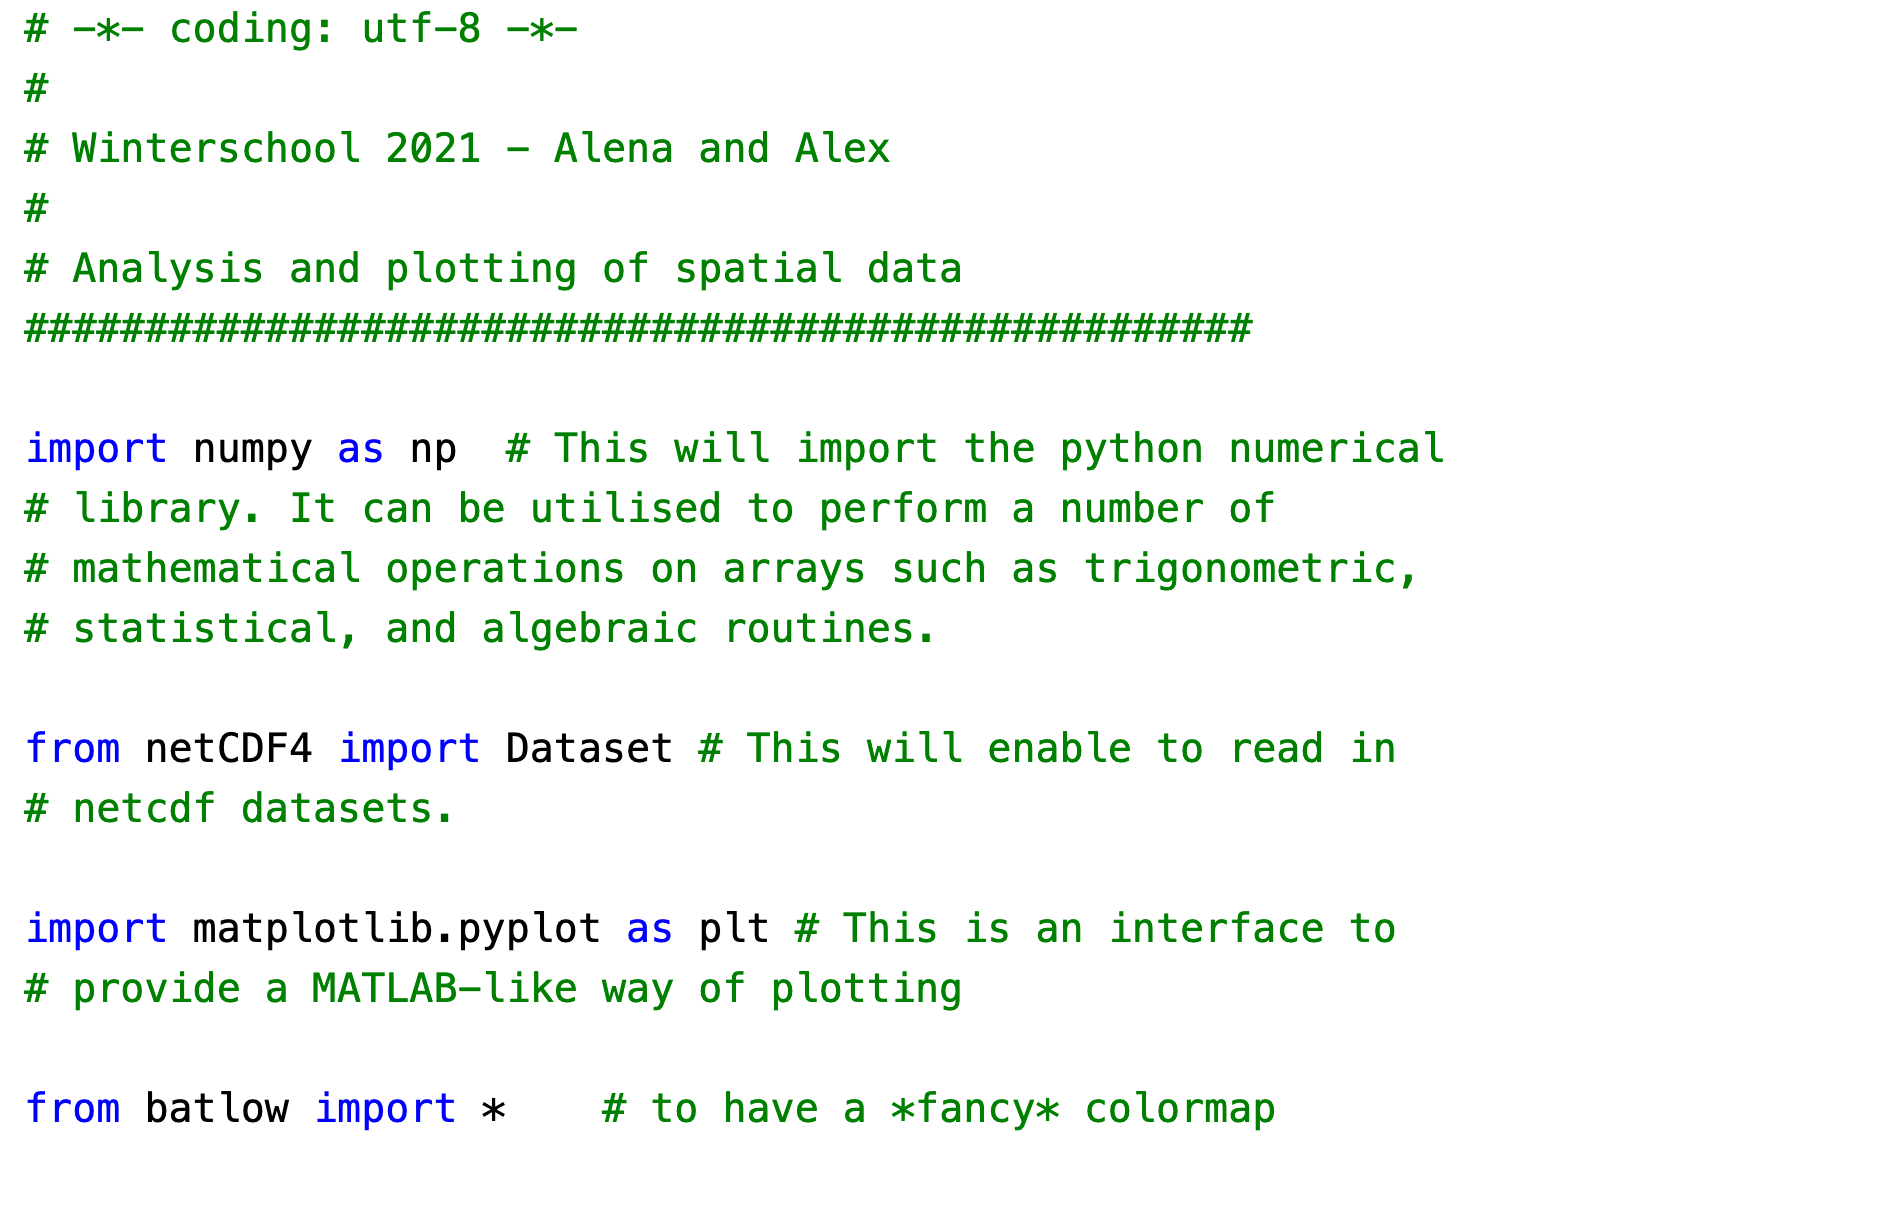
\includegraphics[scale=0.35]{images/Script1_step1.png}}
\end{frame}
 
 
\begin{frame}{\insertsectionnumber{ |} Load into Python and visualise - read a netCDF} 
    Let's import the netcdf dataset and get a sense of the dimensions:\\
        \vspace{0.5cm}
    
\includegraphics[scale=0.35]{images/Script1_step2.png}
        \vspace{2cm}
    (24, 33, 180, 360)
    \begin{beamerboxesrounded}[lower=gray,shadow=true]{Pop quiz:\\
       To which dimensions do these numbers correspond?}
    \end{beamerboxesrounded}
\end{frame}
 
 
\begin{frame}{\insertsectionnumber{ |} Load into Python and visualise - read a netCDF}
    Let's get the dimensions we want and plot the data:\\
        \vspace{0.5cm}
    we want to look at the surface, first time step and whole spatial extent of the file
        \vspace{0.5cm}
    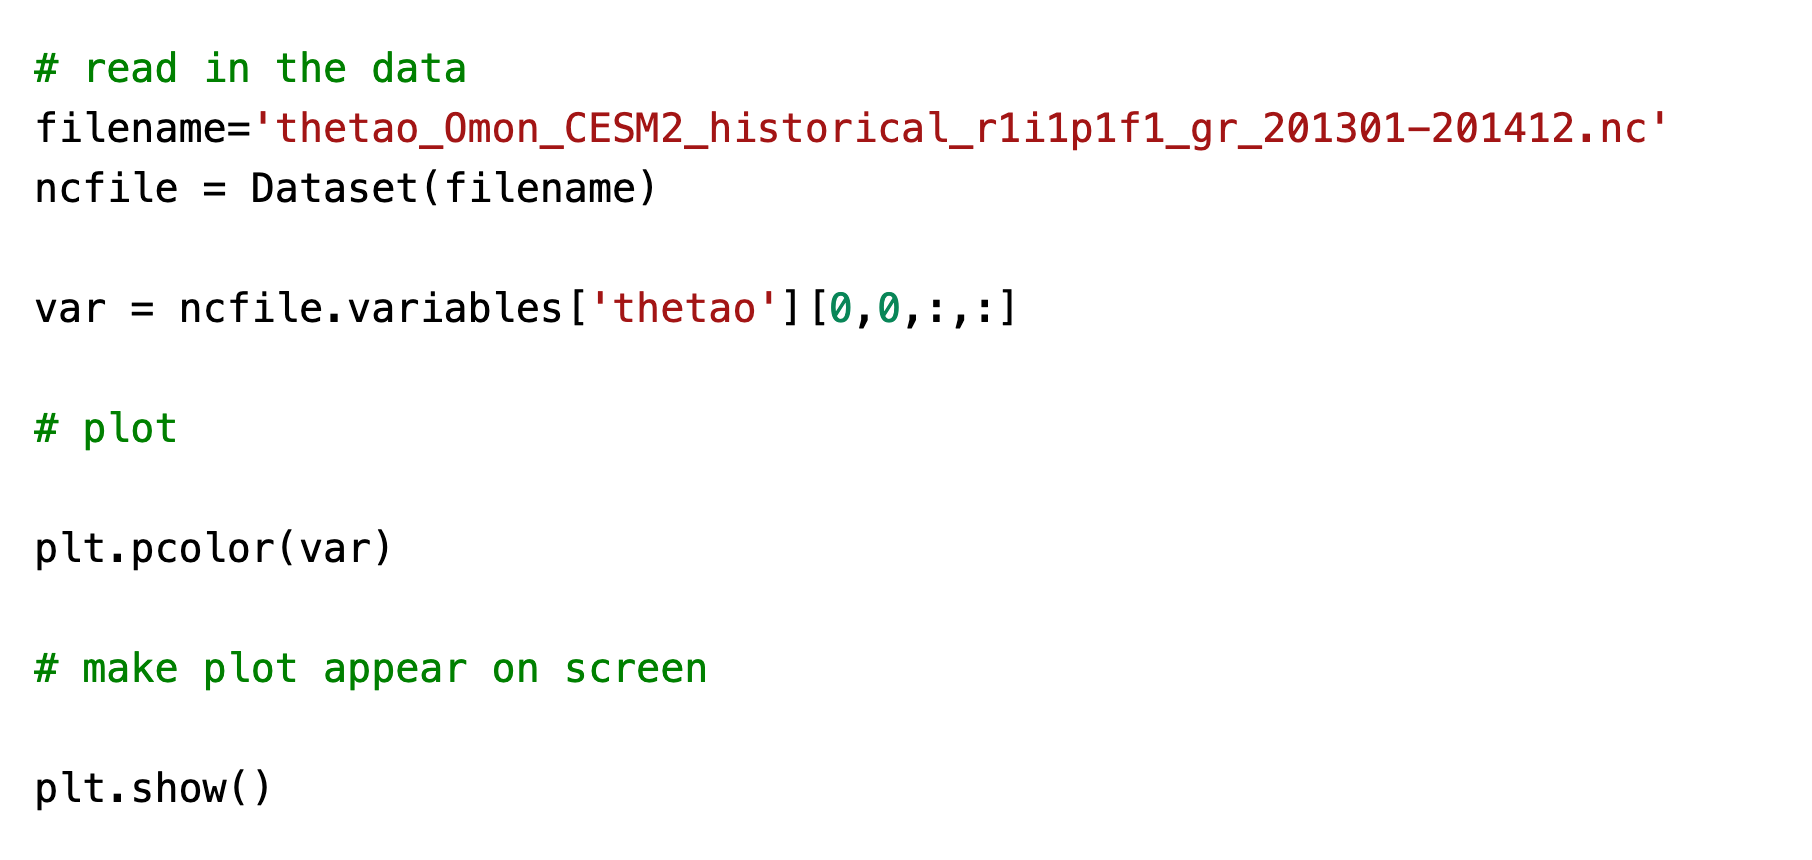
\includegraphics[scale=0.35]{images/Script1_step3.png}
\end{frame}
 
 
\begin{frame}{\insertsectionnumber{ |} Load into Python and visualise - simple plot} 
    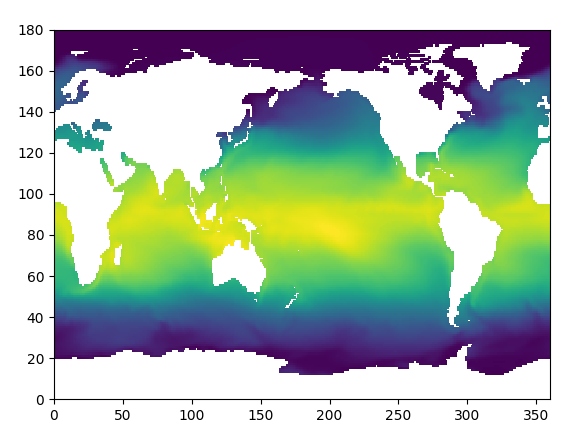
\includegraphics[scale=0.45]{images/script1_fig1.png}
\end{frame}
 
  
\begin{frame}{\insertsectionnumber{ |} Load into Python and visualise - simple plot} 
    Let's add the latitude and longitude coordinates:\\
        \vspace{0.5cm}
    
\includegraphics[scale=0.35]{images/Script1_step4.png}
\end{frame}
  
  
\begin{frame}{\insertsectionnumber{ |} Load into Python and visualise - simple plot} 
    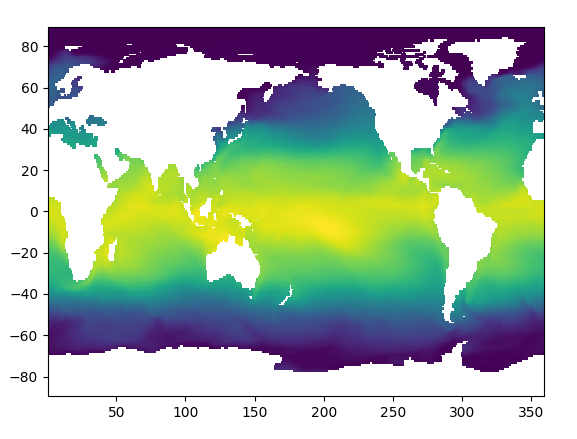
\includegraphics[scale=0.45]{images/Script1_fig2.png}
\end{frame}
 
 
\begin{frame}{\insertsectionnumber{ |} Load into Python and visualise - colormap} 
    
\includegraphics[scale=0.35]{images/Nature.png}\\
        \vspace{0.5cm}
     Let's add a *fancy* colormap:\\
    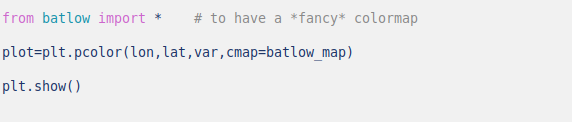
\includegraphics[scale=0.35]{images/Script1_step5.png}\\
        \vspace{0.3cm}
    (!! we need to add the batlow.py to the working directory)\\
\end{frame}
 
 
\begin{frame}{\insertsectionnumber{ |} Load into Python and visualise - colormap} 
    \vspace{0.5cm}
    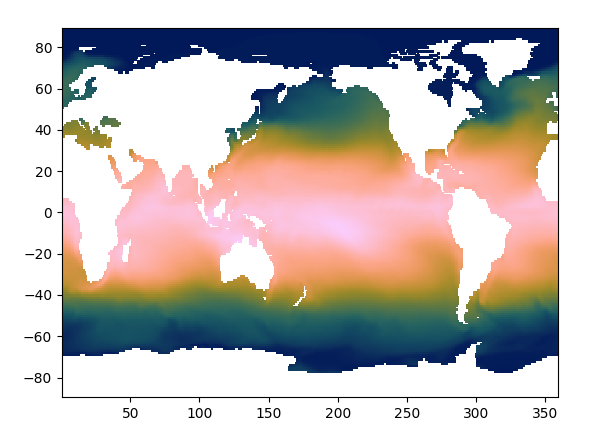
\includegraphics[scale=0.45]{images/Script1_fig3.png}
\end{frame}
 
 
\begin{frame}{\insertsectionnumber{ |} Load into Python and visualise - colormap} 
    \vspace{0.5cm}
    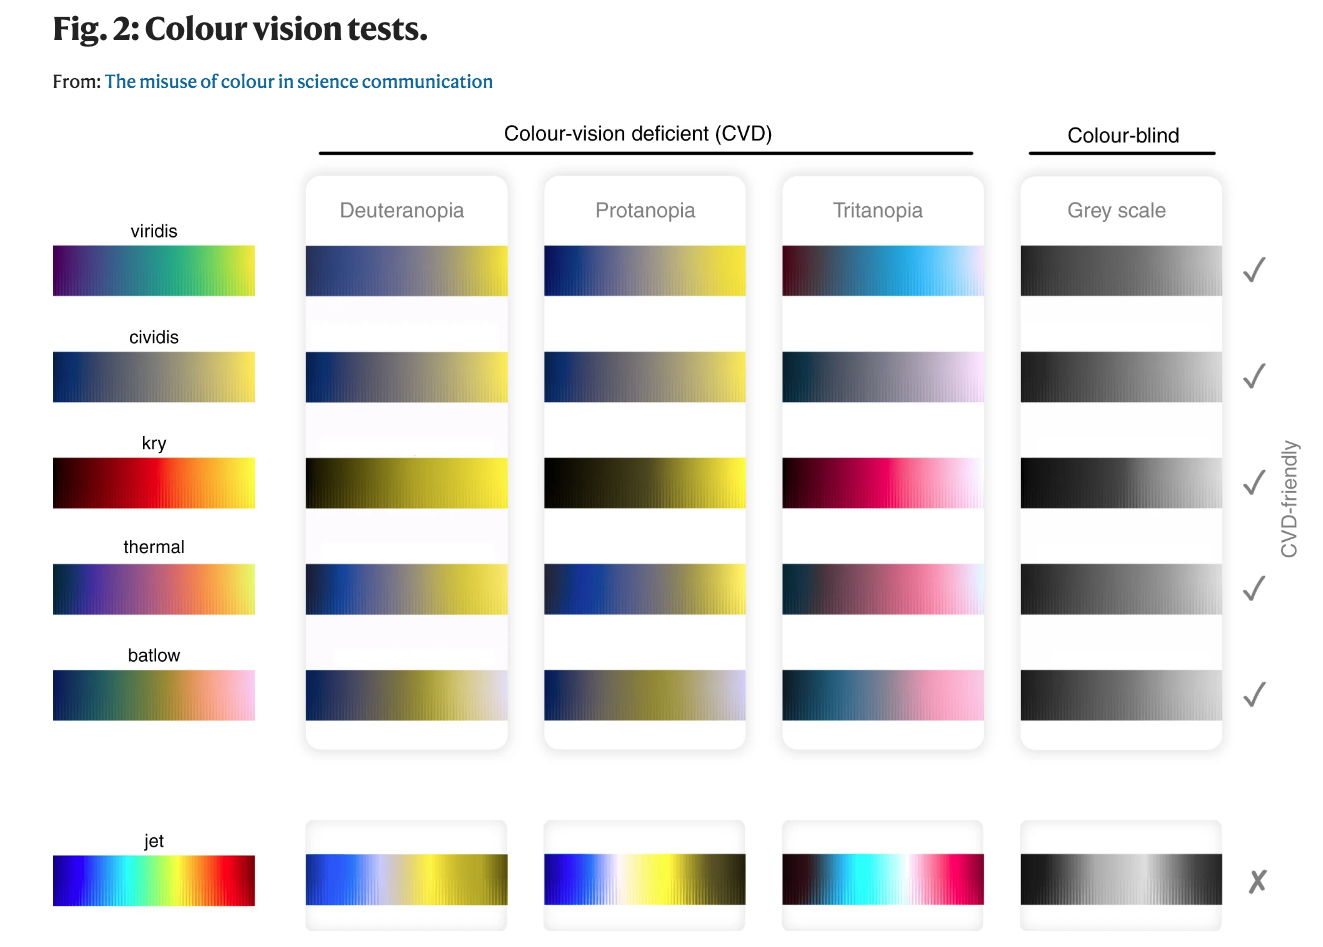
\includegraphics[scale=0.20]{images/Colormap_1.png}
\end{frame}
 
 
\begin{frame}{\insertsectionnumber{ |} Load into Python and visualise - colormap}
    \vspace{0.5cm}
    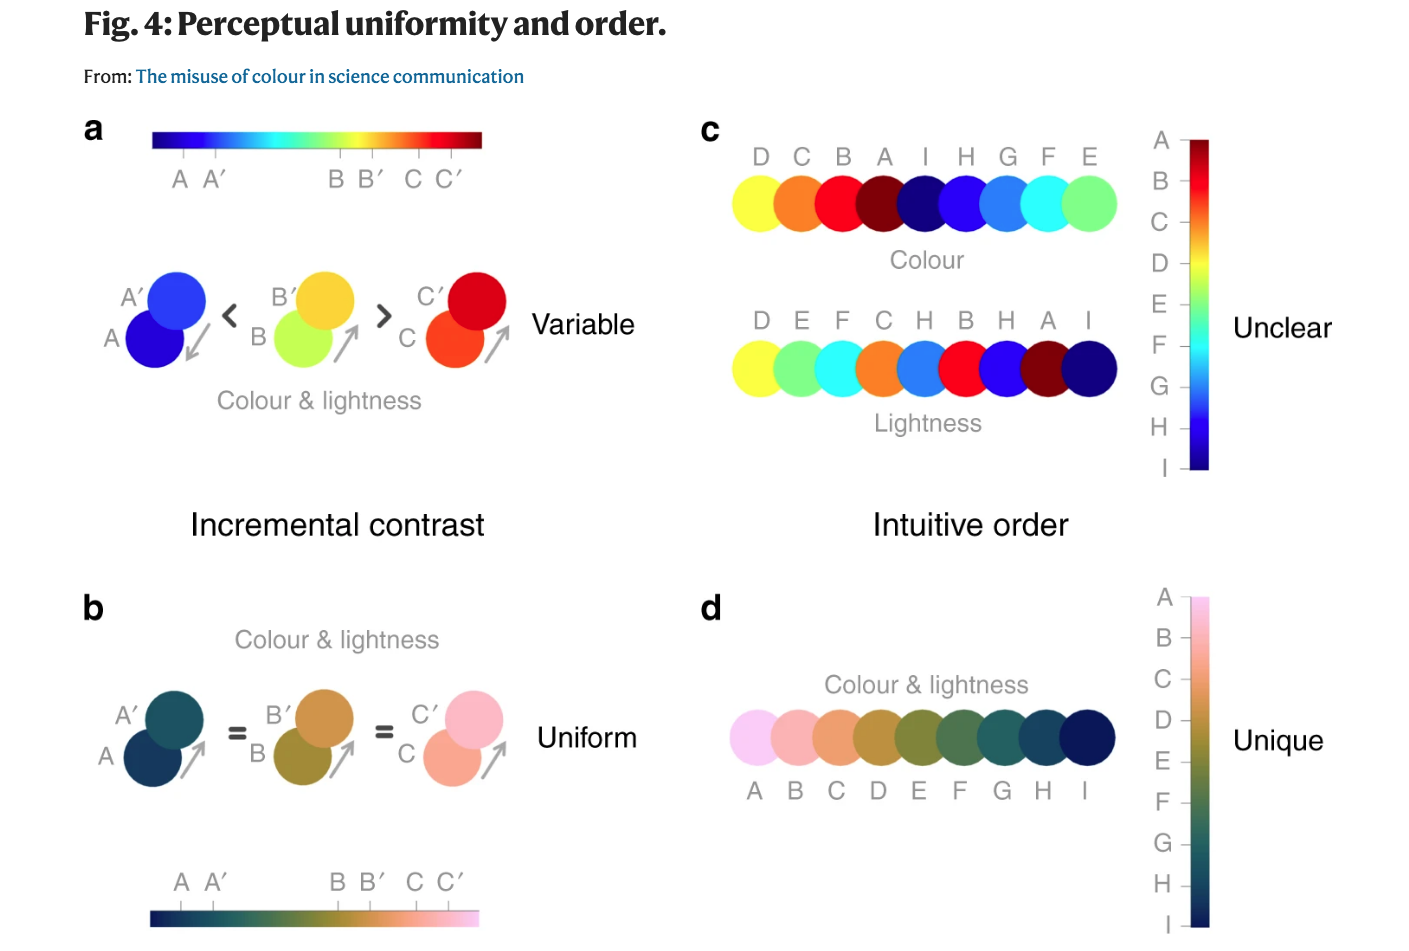
\includegraphics[scale=0.20]{images/Colormap_2.png}
\end{frame}
  
\begin{frame}{\textbf{3 |} Load into Python and visualise - colormap} 
    \vspace{0.5cm}
    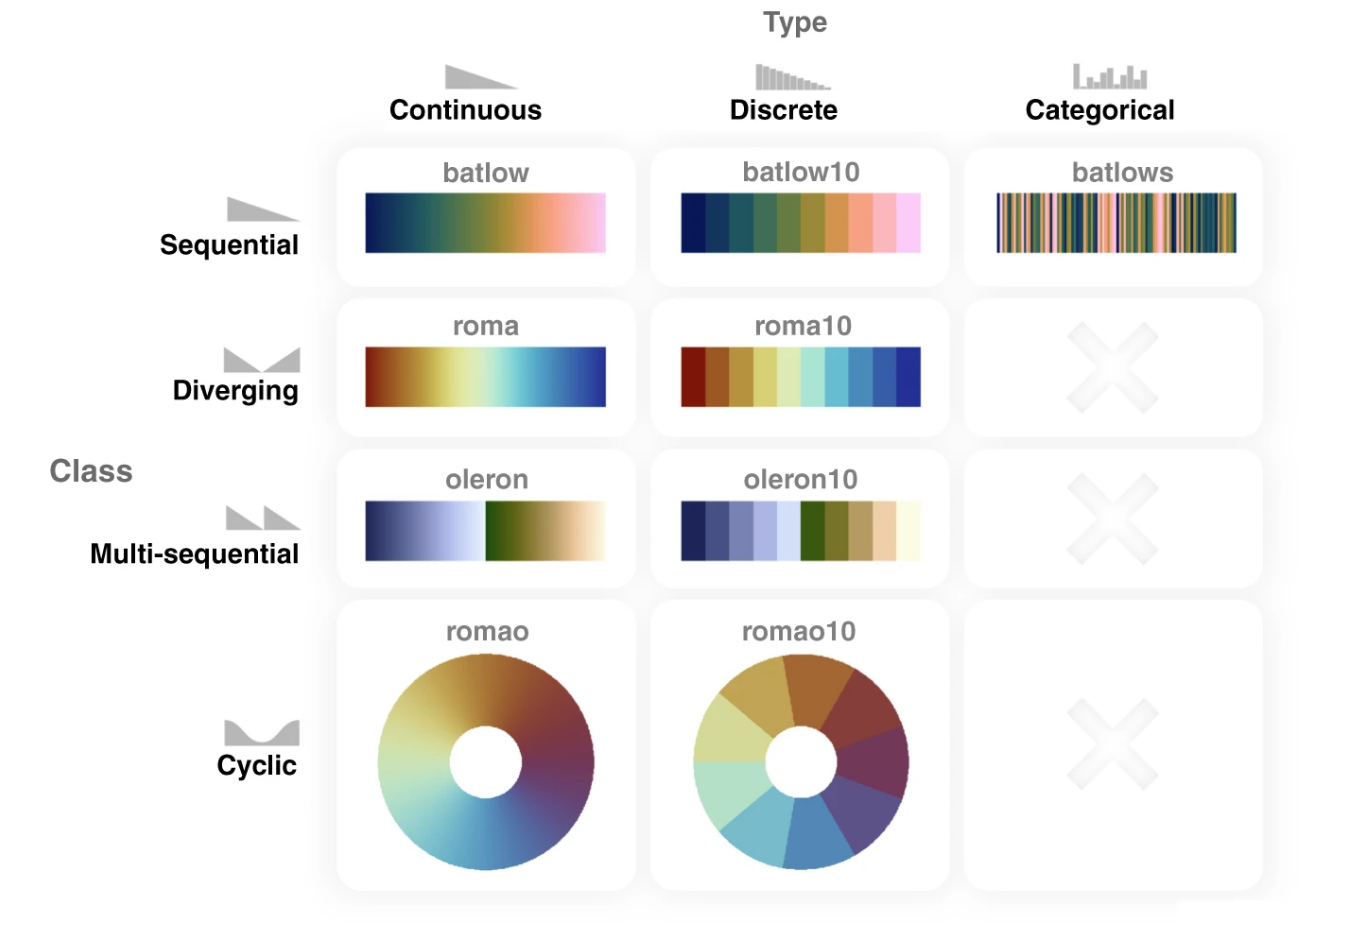
\includegraphics[scale=0.20]{images/Colormap_3.png}
\end{frame}
  
  
 
\begin{frame}{\insertsectionnumber{ |} Load into Python and visualise - labels and colorbar} 
    Let's add labels and a colorbar limited at 20$^{\circ}$C, but pay attention to the variable names and units!
        \vspace{0.5cm}
    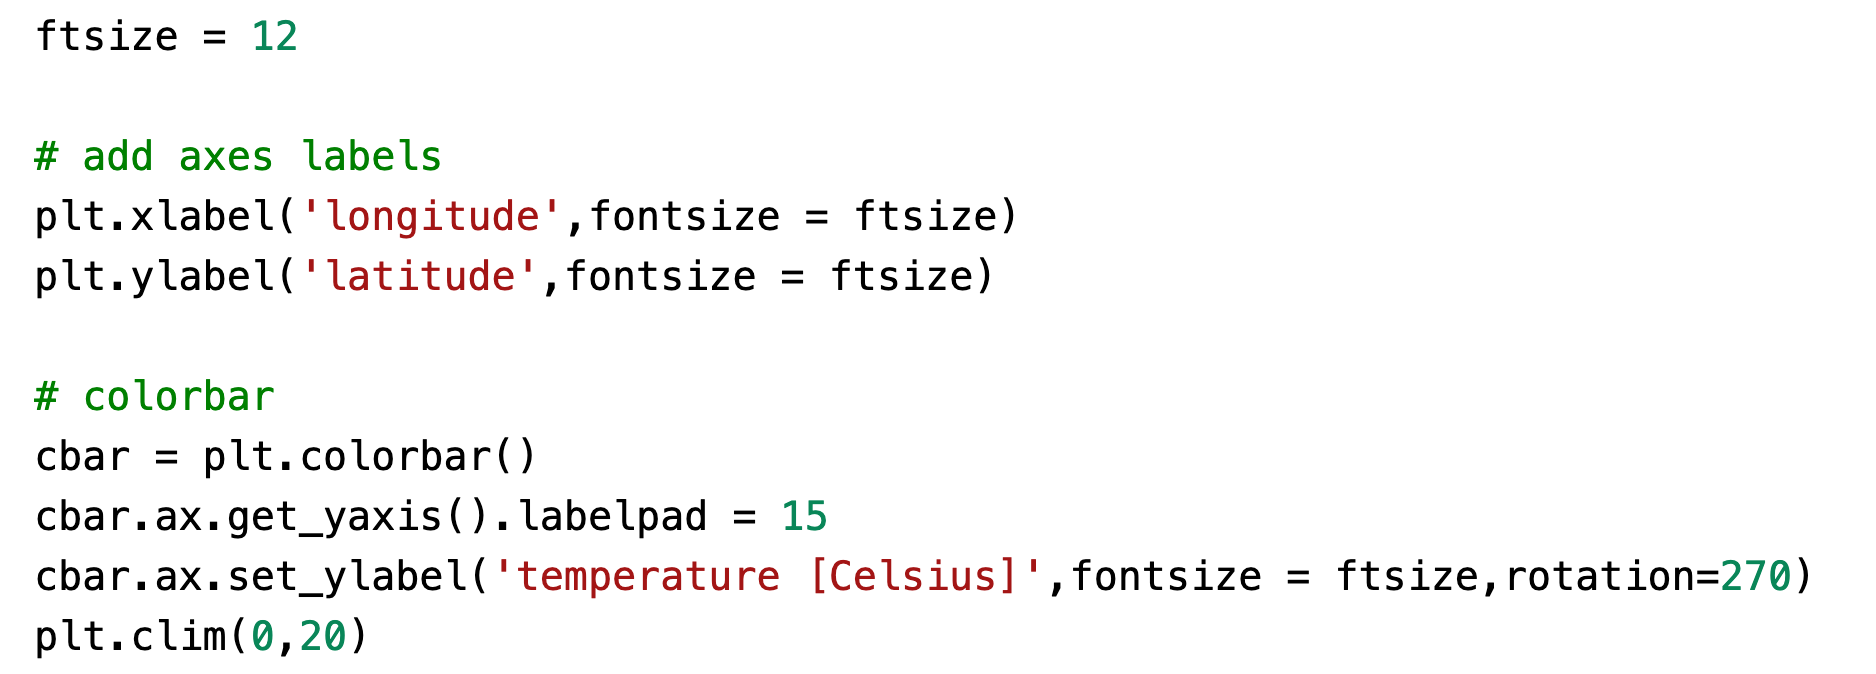
\includegraphics[scale=0.35]{images/Script1_step6.png}
\end{frame}
 
 
\begin{frame}{\insertsectionnumber{ |} Load into Python and visualise - labels and colorbar} 
        \vspace{0.5cm}
    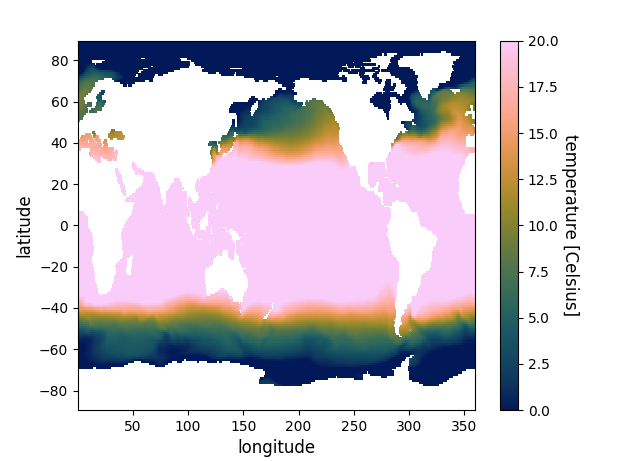
\includegraphics[scale=0.45]{images/Script1_fig4.png}
\end{frame}
 
 
\begin{frame}{\insertsectionnumber{ |} Load into Python and visualise - masking} 
    And, if we wanted to mask out some data, we can use \textbf{cdo} as done previously\\
    But it is also possible in python:\\
        \vspace{0.2cm}
    To mask out a certain value:\\
    
\includegraphics[scale=0.35]{images/Script1_step7.png}\\
        \vspace{0.5cm}
    and to mask an area based on lon/lat:
        \vspace{0.2cm}
    lon and lat are 1D variables, we need to make them 2D first:
    
\includegraphics[scale=0.35]{images/Script1_step8.png}  
        \vspace{0.3cm}
\end{frame}
 
  
\begin{frame}{\insertsectionnumber{ |} Load into Python and visualise - masking} 
    \begin{columns}
        \column[c]{6.5cm}
        To mask out a certain value:
            \vspace{0.5cm}
        \centering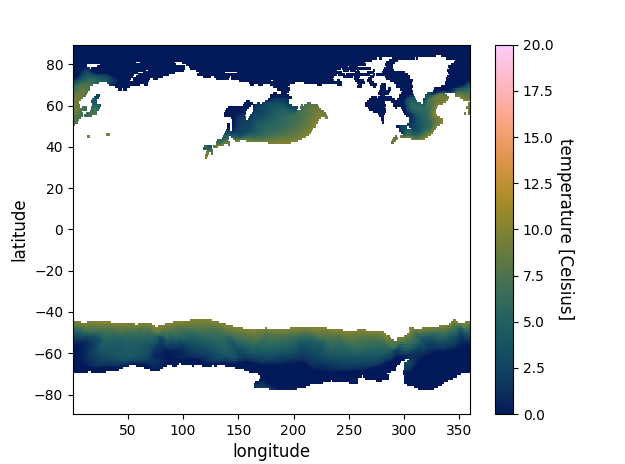
\includegraphics[scale=0.25]{images/Script1_fig5.png}
            \vspace{0.5cm}
        \column[c]{6.5cm}
        and to mask an area based on lon/lat:
            \vspace{0.3cm}
        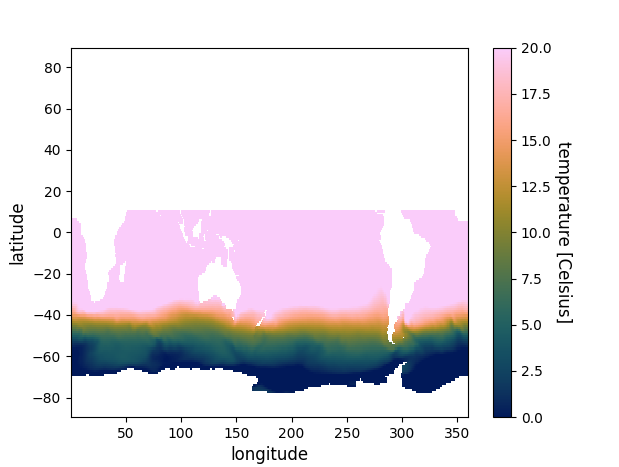
\includegraphics[scale=0.25]{images/Script1_fig6.png}
            \vspace{0.3cm}
    \end{columns}
\end{frame}

%###################################################################
 
\begin{frame}{\insertsectionnumber{ |} Load into Python and visualise - cross-sections}
    We swap dimensions and plot along two dimensions (lon/time, depth/time,...).\\
        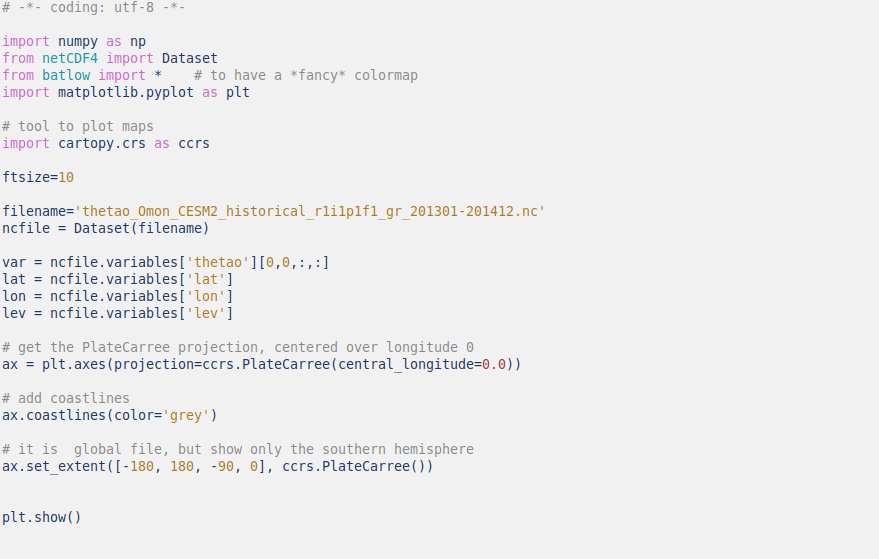
\includegraphics[scale=0.35]{images/Script2_step1.png}
\end{frame}
          
          
\begin{frame}{\insertsectionnumber{ |} Load into Python and visualise - cross-sections}
    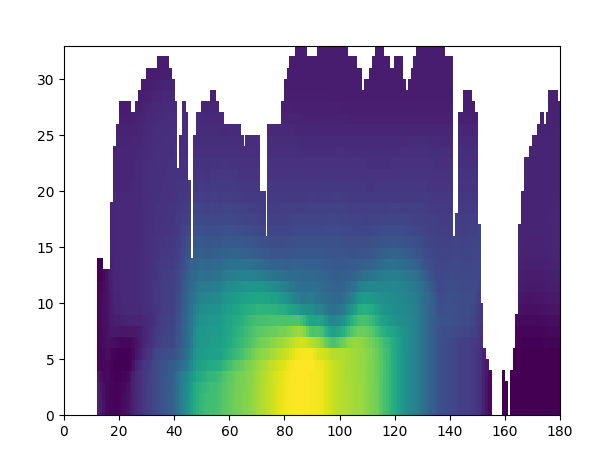
\includegraphics[scale=0.45]{images/Script1_fig7.png}
\end{frame}
 
  
\begin{frame}{\insertsectionnumber{ |} Load into Python and visualise - cross-sections}
    To reverse the plot:\\
    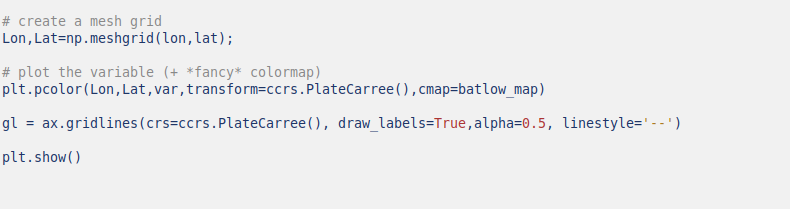
\includegraphics[scale=0.35]{images/Script2_step2.png}\\
    And add labels, colorbar,...
    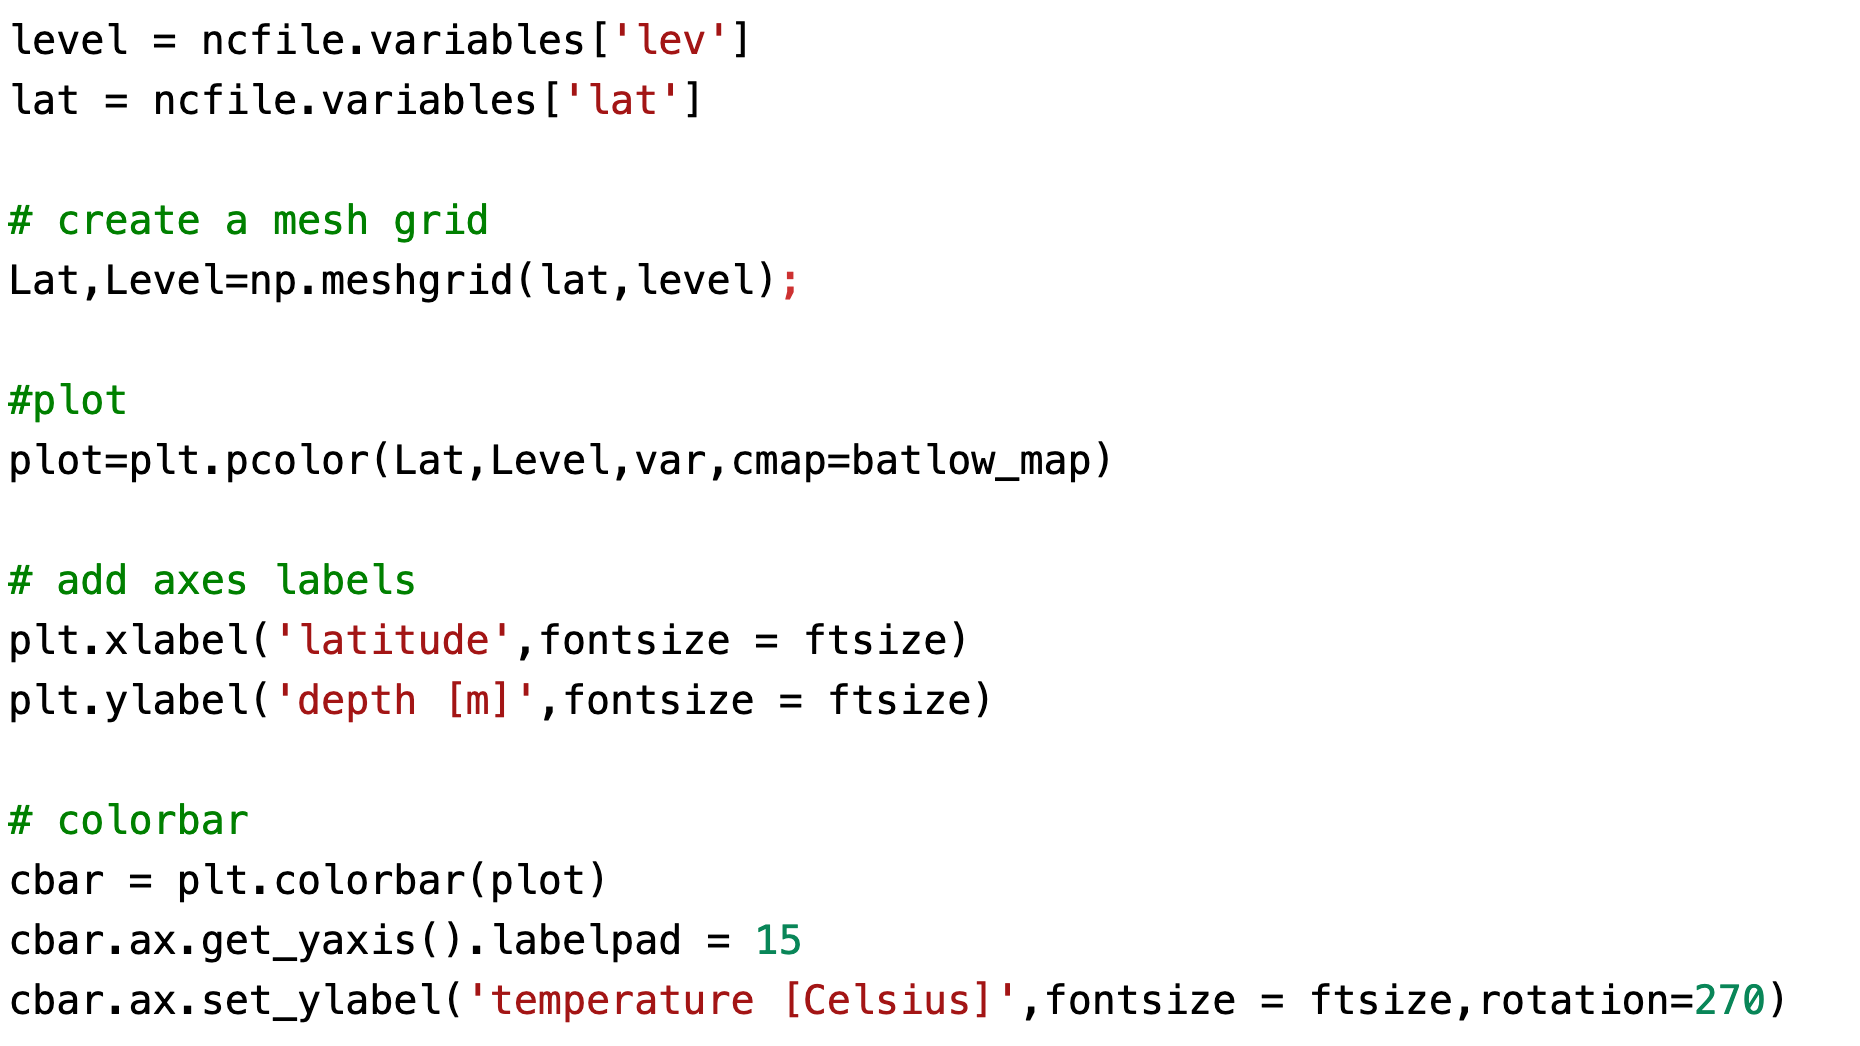
\includegraphics[scale=0.35]{images/Script2_step3.png}
\end{frame}
 
 
\begin{frame}{\insertsectionnumber{ |} Load into Python and visualise - cross-sections} 
    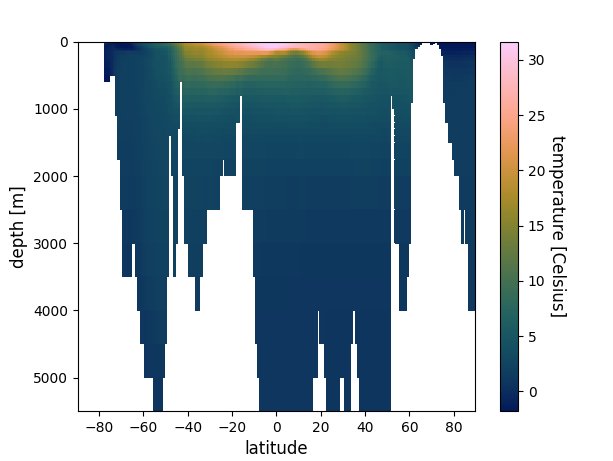
\includegraphics[scale=0.45]{images/script1_fig8.png}
\end{frame}


\begin{frame}{\insertsectionnumber{ |} Load into Python and visualise - cross-sections}
    And finally add contour lines:\\
    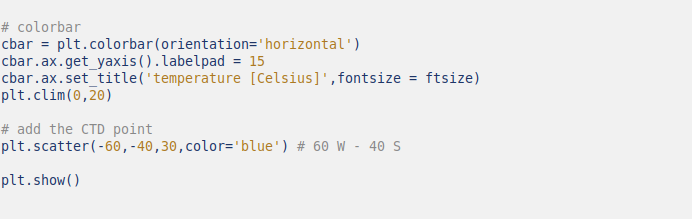
\includegraphics[scale=0.35]{images/Script2_step4.png}\\
\end{frame}


\begin{frame}{\insertsectionnumber{ |} Load into Python and visualise - cross-sections}
    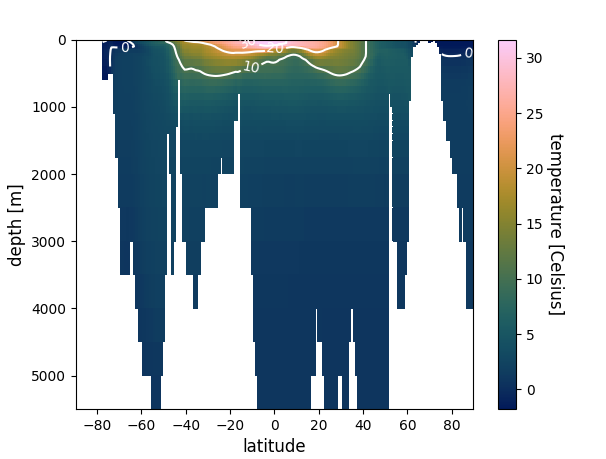
\includegraphics[scale=0.45]{images/script1_fig9.png}
\end{frame}

% ####################################################################

\begin{frame}{\insertsectionnumber{ |} Load into Python and visualise - time-depth diagram} 
    Let's plot one location over time, with depth: \\
    \hbox{\hspace{-0.5cm}\includegraphics[scale=0.35]{images/Script3_step1.png}}
\end{frame}


\begin{frame}{\insertsectionnumber{ |} Load into Python and visualise - time-depth diagram} 
    Let's plot one location over time, with depth: \\
    \hbox{\hspace{-0.5cm}\includegraphics[scale=0.35]{images/Script3_step2.png}}
\end{frame}


\begin{frame}{\insertsectionnumber{ |} Load into Python and visualise - time-depth diagram} 
    \includegraphics[scale=0.45]{images/script1_fig10.png}
\end{frame}


\begin{frame}{\insertsectionnumber{ |} Load into Python and visualise - pop quiz}
    \begin{beamerboxesrounded}[lower=gray,shadow=true]{Pop quiz:\\
        \begin{itemize}
            \item Try to find another location (different hemisphere or equator),\\
            or change the depth range on the y-axis.
            \item Do an horizontal section along the equator / 30$^{\circ}$S with depth values. \\
            Compare the extent of the mixed layers
        \end{itemize}}
    \end{beamerboxesrounded}
\end{frame} 

%*****************************************************************
% SEC4 |Make a publication figure
%*****************************************************************

\begin{frame}{\insertsectionnumber{ |} Make a publication figure}
    Now that we have a pretty figure, let's start being fancy.\\
        \vspace{0.3cm}
%    Mapping is the \textbf{second} step, not the first!\\
%        \vspace{0.5cm}
    We will use the \href{https://scitools.org.uk/cartopy/docs/latest/}{\beamerbutton{\Huge{cartopy}}} package:\\
    \includegraphics[scale=0.35]{images/Script4_step1.png}
\end{frame}


\begin{frame}{\insertsectionnumber{ |} Make a publication figure - cartopy}
    Let's plot SST at the surface, over the whole domain with the 'Plate Carree" projection
        \includegraphics[scale=0.35]{images/Script4_step2.png}
\end{frame}
  
  
\begin{frame}{\insertsectionnumber{ |} Make a publication figure - cartopy} 
    \includegraphics[scale=0.50]{images/script2_fig1.png}
\end{frame}


\begin{frame}{\insertsectionnumber{ |} Make a publication figure - cartopy} 
    Let's fill in the variable, but lat and lon have to be  2D (use meshgrid)
    \includegraphics[scale=0.35]{images/Script4_step3.png}
\end{frame}


\begin{frame}{\insertsectionnumber{ |} Make a publication figure - cartopy} 
    \includegraphics[scale=0.50]{images/script2_fig2.png}
\end{frame}
 
 
\begin{frame}{\insertsectionnumber{ |} Make a publication figure - cartopy} 
    Let's format the axes:
    \includegraphics[scale=0.35]{images/Script4_step4.png}
\end{frame}


\begin{frame}{\insertsectionnumber{ |} Make a publication figure - cartopy} 
    \includegraphics[scale=0.50]{images/script2_fig3.png}
\end{frame}


\begin{frame}{\insertsectionnumber{ |} Make a publication figure - cartopy}
    Imagine: \\
    \begin{itemize}
        \item we have a CTD station (at 60$^{\circ}$CW 40$^{\circ}$CS and 4500 m depth (30th level)) 
            \vspace{0.3cm}
        \item and let's add the colorbar
    \end{itemize}
    \includegraphics[scale=0.35]{images/Script4_step5.png}
\end{frame}


\begin{frame}{\insertsectionnumber{ |} Make a publication figure - cartopy}
    \includegraphics[scale=0.60]{images/script2_fig4.png}
\end{frame}

%######## xarray example

\begin{frame}{\insertsectionnumber{ |} Make a publication figure - \textbf{xarray}}
    \href{https://xarray.pydata.org/}{\beamerbutton{\Huge{xarray}}} is an useful package when dealing with netCDFs containing metadata: \\
        \vspace{0.5cm}
    \includegraphics[scale=0.35]{images/xarray_info.png}
\end{frame}


\begin{frame}{\insertsectionnumber{ |} Make a publication figure - \textbf{xarray}}
    \includegraphics[scale=0.45]{images/xarray_1.png}
\end{frame}


\begin{frame}{\insertsectionnumber{ |} Make a publication figure - \textbf{xarray}}
    \includegraphics[scale=0.35]{images/print_xarray.png}
\end{frame}


\begin{frame}{\insertsectionnumber{ |} Make a publication figure - \textbf{xarray}}
    \includegraphics[scale=0.35]{images/xarray_2.png}
\end{frame}

\begin{frame}{\insertsectionnumber{ |} Make a publication figure - \textbf{xarray}}
The title, colorbar,.. are automatically added:\\
    \includegraphics[scale=0.50]{images/figure_xarray.png}
\end{frame}

%###########
\begin{frame}{\insertsectionnumber{ |} Make a publication figure - difference between two datasets in \textbf{cdo}}
    What if we want to compare two datasets, which are not on the same grid? \\
        \vspace{0.5cm}
    Re-Mapping is the answer !\\
        \vspace{0.5cm}
    We can do it in \textbf{cdo}: \\
    \textit{cdo remapbil ...} will use bilinear interpolation to remap one grid ont another \\
    (! create a grid description file using \textit{cdo griddes} beforehand)\\
\end{frame}


\begin{frame}{\insertsectionnumber{ |} Make a publication figure - difference between two datasets in \textbf{cdo}}
    Get the grid description of the file you want to remap \textbf{onto}: (here, ERA5)\\
        \vspace{0.5cm}
    \textcolor{black}{cdo griddes SST\_ERA5\_201301.nc > grid\_era5.txt}\\
        \vspace{0.5cm}
    \includegraphics[scale=0.35]{images/Script5_step0.png}
\end{frame}
  
  
\begin{frame}{\insertsectionnumber{ |} Make a publication figure - difference between two datasets in \textbf{cdo}} 
    Then: 
        \begin{itemize}
            \item we remap using a bilinear interpolation: \\
                \textcolor{black}{cdo remapbil,grid\_era5.txt thetao\_Omon\_CESM2\_historical\_r1i1p1f1\_gr\_201301-201412.nc theta\_remapped.nc}
                    \vspace{0.3cm}
            \item  to subtract one from the other, the two files have to have the 'same variable' (name):\\
                \textcolor{black}{cdo chname,thetao,sst theta\_remapped.nc theta\_remapped\_sst.nc} \\
                    \vspace{0.3cm}
            \item and subtract the two files:\\
                \textcolor{black}{cdo sub SST\_ERA5\_201301.nc theta\_remapped\_sst.nc diff\_era5\_theta.nc} \\
                    \vspace{0.3cm} 
            \item let's check the nc file, and play with the colorbar, range,...
        \end{itemize}
\end{frame}

  
\begin{frame}{\insertsectionnumber{ |} Make a publication figure - remap with griddata} 
    Now, let's do the same in Python !\\
        \vspace{0.3cm} 
    We will use the \textbf{griddata package}\\
    \includegraphics[scale=0.35]{images/Script5_step1.png}
\end{frame}


\begin{frame}{\insertsectionnumber{ |} Make a publication figure - remap with griddata} 
    And it needs the data to be formatted in a specific way:
    \includegraphics[scale=0.35]{images/Script5_step2.png}
\end{frame}


\begin{frame}{\insertsectionnumber{ |} Make a publication figure - remap with griddata}
    And it needs the data to be formatted in a specific way:
    \includegraphics[scale=0.35]{images/Script5_step3.png}
\end{frame}


\begin{frame}{\insertsectionnumber{ |} Make a publication figure - make different subplots} 
    Let's make 3 subplots in the figure: 
    \begin{itemize}
        \item the ERA5 data
        \item the CMIP regridded data
        \item the difference between the two
    \end{itemize}
        \vspace{0.5cm}
    \includegraphics[scale=0.35]{images/Script5_step4.png}
\end{frame}


\begin{frame}{\insertsectionnumber{ |} Make a publication figure - make different subplots} 
    \includegraphics[scale=0.55]{images/script5_fig2.png}
        \vspace{0.3cm}
\end{frame}


\begin{frame}{\insertsectionnumber{ |} Make a publication figure - make different subplots} 
    Add the colorbars : \\
    \begin{itemize}
        \item batlow, but same limits as the second subplot
            \vspace{0.3cm}
        \item batlow, but same limits as the first subplot
            \vspace{0.3cm}
        \item red-blue (the vik colorbar)!
    \end{itemize}
    \vspace{0.3cm}
    Hint: we can print out the min and max values of our variables :
    \includegraphics[scale=0.35]{images/hint.png}\\
\end{frame}

\begin{frame}{\insertsectionnumber{ |} Make a publication figure - make different subplots} 
    \includegraphics[scale=0.35]{images/Script5_step5.png}
\end{frame}


\begin{frame}{\insertsectionnumber{ |} Make a publication figure - make different subplots} 
    And to center the vik colorbar around 0 : \\
        \vspace{0.3cm}
    \includegraphics[scale=0.35]{images/Script5_step6.png}
\end{frame}


\begin{frame}{\insertsectionnumber{ |} Make a publication figure - make different subplots} 
    And to center the vik colorbar around 0: \\
        \vspace{0.3cm}
    (hint: find out the min and max values) \\
        \vspace{0.3cm}
    \includegraphics[scale=0.35]{images/Script5_step7.png}
\end{frame}


\begin{frame}{\insertsectionnumber{ |} Make a publication figure - make different subplots} 
    \centering\includegraphics[scale=0.25]{images/script5_fig3.png}
    \begin{beamerboxesrounded}[lower=gray,shadow=true]{
        Pop quiz:\\
        Our figure will \textbf{not} look like this, find out why and fix it!}
    \end{beamerboxesrounded}
\end{frame}


\begin{frame}{\insertsectionnumber{ |} Make a publication figure - save the figure} 
    Finally, let's set the layout and save the figure: \\
        \vspace{0.3cm}
    \includegraphics[scale=0.35]{images/Script5_step8.png}
\end{frame}


\begin{frame}{\insertsectionnumber{ |} Make a publication figure - pop quiz} 
    \begin{beamerboxesrounded}[lower=gray,shadow=true]{
        Pop quiz: \\
            \vspace{0.3cm}
        Let's do the same as for the final \textit{cdo} command, but in a python script:\\
            \begin{itemize}
                \item two cross sections
                    \vspace{0.15cm}
                \item of mean June
                    \vspace{0.15cm}
                \item sea surface temperature
                    \vspace{0.15cm}
                \item over the dateline
                    \vspace{0.3cm}
                \item using the two thetao files (201301-201412 and 185001-185112)
                    \vspace{0.15cm}
                \item using the red-blue colormap
                    \vspace{0.15cm}
                \item with the surface at the top 
                    \vspace{0.15cm}
                \item and a colorbar symmetrical around 0
            \end{itemize}
                \vspace{1.5cm}}
    \end{beamerboxesrounded}
\end{frame}


\begin{frame}{\insertsectionnumber{ |} Make a publication figure - pop quiz} 
    \centering\includegraphics[scale=0.22]{images/script6_fig1.png}\\
\end{frame}


\begin{frame}{\insertsectionnumber{ |} Make a publication figure - pop quiz}
    \begin{columns}
        \column[c]{5.5cm}
            And as a final check,\\
                \vspace{0.3cm}
             load your cdo final result and \\
                \vspace{0.3cm}
             compare to the output of this script! 
        \column[c]{6.5cm}             
            \includegraphics[scale=0.22]{images/script6_fig2.png}\\ 
    \end{columns}
\end{frame}

%%%%%%%%%%%%%%%%%%%%%%%% END CONTENT %%%%%%%%%%%%%%%%%%%%%%
\section{Latex}
%\includepdf[pages=-]{LATEX.pdf}


%%%%%%%%%%%%%%%%%%%%%%%% ADD CONTENT %%%%%%%%%%%%%%%%%%%%%%
\section{Work Structure /& Version Control}
% specific header SJ slides
% pengu with E for example, T task, ! take home message
%=============================================================================================
 
\begin{frame}{\insertsectionnumber{ |} Reality Check}
\begin{columns}
\column[c]{5cm}

\begin{beamerboxesrounded}[lower=gray,shadow=true]{
I plotted this real nice figure for Richard a while ago.  Now Peter wants something very similar. The graph just needs a different colormap - easy! \\
But how did I do it?  Wish I used a damn script and saved it ...
}
\end{beamerboxesrounded}
% work with scripts and save them with your figure
\vspace*{0.2cm}
\begin{beamerboxesrounded}[lower=gray,shadow=true]{
I wrote this really flash paragraph about Extra-Terrestian fossils in my samples. Rob thought it was bogus.  Now that they have landed in Area 51 to collect their trash I would really like that paragraph back in the maunscript. 
}
\end{beamerboxesrounded}
% version control, backup
\begin{itemize}
\item How do you work?
\item What is your workflow?
\item Does your work structure map your workflow?
\end{itemize}

\column[c]{5cm}

\begin{beamerboxesrounded}[lower=gray,shadow=true]{
I just discovered a really cool feature in one of the 50+ simulations from last year. \\
What was the vertical diffusion I used in that simulation? And how warm was the atmospheric forcing data?
}
\end{beamerboxesrounded}
% naming convention, backup

\vspace*{0.2cm}
\begin{beamerboxesrounded}[lower=gray,shadow=true]{
Lockdown was fun - got lots of processing and writing done. Will copy and backup files when I get back to the office next week. \\
My labtop dropped off the table last night. The hard drive is jammed.
}
\end{beamerboxesrounded}
% instant backup

\vspace*{0.2cm}
\begin{beamerboxesrounded}[lower=gray,shadow=true]{
Finally got around to publish some of that ancient thesis material from 5 years ago.  Just got an email from the journal's editor, requesting the 6 figures in high res.
}
\end{beamerboxesrounded}
\vspace{0.2cm} \hspace{1cm}
\includegraphics[height=2.0cm]{./images/fishbones.jpg} \hspace{-0.2cm} \includegraphics[height=0.8cm]{./images/brokencomputer.jpg}
%\end{itemize}
\end{columns}
\end{frame}

%=============================================================================================
%
%\begin{frame}{\insertsectionnumber{ |} Reality Check}
%\begin{columns}
%\column[c]{5cm}
%% 
%\begin{beamerboxesrounded}[lower=gray,shadow=true]{
%Plotting Scripts \\
%  
%Naming  \\
%  
%Backup \\
%  
%}
%\end{beamerboxesrounded}
%%% work with scripts and save them with your figure
%\vspace*{0.2cm}
%
%\begin{beamerboxesrounded}[lower=gray,shadow=true]{
%
%
%Version Control \\
%
%
%Backup \\
%
%
%}
%\end{beamerboxesrounded}
%%% version control, backup
%
%\column[c]{5cm}
%%
%\begin{beamerboxesrounded}[lower=gray,shadow=true]{
%Naming \\
%
%
%Data Handling \\
%
%
%Folder Structure \\
%}
%\end{beamerboxesrounded}
%%% naming convention, backup
%%
%\vspace*{0.2cm}
%\begin{beamerboxesrounded}[lower=gray,shadow=true]{
%Instant Backup \\
%Cross Desk syncronization
%}
%\end{beamerboxesrounded}
%%% instant backup
%%
%\vspace*{0.2cm}
%\begin{beamerboxesrounded}[lower=gray,shadow=true]{
%Backup \\
%
%Naming \\
%
%Version Control \\
%
%
%Plotting Scrits \\
%
%ARchiving \\
%}
%\end{beamerboxesrounded}
%%
%%
%\end{columns}
%\begin{itemize}
%\item How do you work?
%\end{itemize}
%\end{frame}

%=============================================================================================
%
\begin{frame}{\insertsectionnumber{ |} Workflow}
\begin{itemize}
\item \textbf{What is a workflow?} \\
Wikipedia \\
\textit{"A workflow consists of an orchestrated and \textbf{repeatable} pattern of activity, enabled by the systematic organization of resources into processes that transform matericals, provide services, or process information."} \\

\item Examples \\
\item[\textbullet] All physical and mental steps between your hypothesis and the published result. \\
\item[\textbullet] All related tasks and stages to carry out an experiment. \\
\item[\textbullet]All activities, materials and documents to measure a rock sample.


\end{itemize}

\begin{columns}

\column[c]{7.5cm}

\begin{itemize}

\item \textbf{Why do we need to think about our workflows?}

\item Repeatability and reproducability are key requirements in science. For example \\
\begin{itemize}

\item[\textbullet] Result of a numerical model. \\
\item[\textbullet] Chemical analysis of a rock sample. \\
\item[\textbullet] Pre-processing of a dataset. \\
\item[\textbullet] A figure in a publication. 
\end{itemize}
\item Maximizes work efficiency and increases effectiveness. 
\end{itemize}

\column[c]{2cm}
\includegraphics[height=2.6cm]{./images/walkman.jpg}

\end{columns}

\end{frame}

%=============================================================================================
\begin{frame}{\insertsectionnumber{ |} Workflow - a simple concept}

\hspace{2cm}
\begin{beamerboxesrounded}[lower=gray,shadow=true]{
\begin{columns}

\column[c]{3cm}
\footnotesize{
\textbf{State} \\
Product \\
Result \\
Milestone \\
Information \\
Resource 
}

\column[c]{3cm}
\footnotesize{
File \\
Figure \\
data set \\
Sample \\
Accepted publication \\
document 
}
\end{columns}
}
\end{beamerboxesrounded}

\begin{columns}
\column[c]{3cm}
\begin{beamerboxesrounded}[lower=gray,shadow=true]{
\footnotesize{
\textbf{Process} \\
Activity \\
Conversion \\
transformation \\
Transition \\
\\
\textbf{Examples} \\
Writing \\
Dissolving a rock sample \\
Cropping a data set \\
Plotting 
}
}
\end{beamerboxesrounded}
\hspace{2cm}

\column[c]{3cm}
\includegraphics[height=4cm]{./images/box_workflow.png}

\column[c]{3cm}


%
\begin{beamerboxesrounded}[lower=gray,shadow=true]{
\footnotesize{
\textbf{Tools} \\
Material \\
support \\
\\
program function \\
Hammer \\
Software \\
Device \\
Computer \\
Solvent \\
Brain
}
}
\end{beamerboxesrounded}

\end{columns}
 



\end{frame}
%=============================================================================================
\begin{frame}{\insertsectionnumber{ |} Workflow - example}

\vspace{0.5cm}
% schematic ?
\begin{itemize}
\item To be inserted Example Slide with schematic "how to set up and run a model and save outputs"\\
%ScheRepeated interpolation of a bathymetry data set onto the target grid takes about 3 minutes
Out of this will fall the terms "folder structure" "data handling" "version control/backup" "naming convention"
which forms the TOC of the talk.
\end{itemize}
 
\vspace{2cm}
\begin{itemize}

\item Think of a small project in the recent past and sketch the associated workflow.
Examples could be: writing a Marsden one pager, set up and run a simulation or 
analyse rocks and record and store the data.

\item Use the concept of State,  Process,  Tool

\end{itemize}

\end{frame}

%=============================================================================================

\begin{frame}{\insertsectionnumber{ |} Work Structure}

\begin{beamerboxesrounded}[lower=gray,shadow=true]{
\begin{itemize}
%\item What is a work structure? \\
\item A suitable \textbf{work structure} is a systematically organized work environment that \textbf{maps} one specific or a group of \textbf{workflows}. \\
\item The guiding principles to arrange the environment into a suitable structure are \\

\begin{itemize}
\item[\textbullet] Reproducability 
\item[\textbullet] Efficiency 
\item[\textbullet] Cost - in units of storage, processing time, computing load, money, FTE
\end{itemize}

\item For computer based environments the work structure typically consists of blocks such as 

\begin{itemize}
\begin{columns}

\column[c]{4cm}

\item[\textbullet] data sets
\item[\textbullet] software \& apps 
\item[\textbullet] compilers \& data language
\item[\textbullet] \textbf{file formats} 
\item[\textbullet] \textbf{version control}
\item[\textbullet] computer hardware 
\item[\textbullet] storage facilities
\column[c]{4cm}

\item[\textbullet] \textbf{backup procedure}
\item[\textbullet] communicaton model
\item[\textbullet] \textbf{folder structure}  
\item[\textbullet] exchange \& transfer protocol
\item[\textbullet] documentation
\item[\textbullet] \textbf{data handling}
\item[\textbullet] credential management


\end{columns}
\end{itemize}
\end{itemize}

}
\end{beamerboxesrounded}

\begin{itemize}
\item A specific work structure consists of a subset of these blocks. They are not absolute definitions and contain a deliberate degree of redundancy.
\item \textbf{The list of building blocks can be used as a stencil to filter out the important aspects in the workflow that need to be incorporated in your work structure.}
\vspace{0.2cm}
\item Find two entities that are important for your work structure and one that is negligible.  
\end{itemize}



\end{frame}

%=============================================================================================
%
\begin{frame}{\insertsectionnumber{ |} Work Structure - discussion}

\begin{itemize}
\item The implementation of a Work Structure can range from installing a plugin in your browser to manage all your online credentials to writing a large bash scripts that automatically synchronize all your Python scripts between your office desktop and your labotp at home.
\item Apart from the three guiding principles there are other motivations for a well organized work structure

\begin{itemize}
\item[\textbullet] the frustration having to recreate something that has been "lost" 
\item[\textbullet] can not afford to loose a good idea 
\item[\textbullet] wasting time to search for something
\end{itemize} 

\item Protect the products of your creativity, things that were made with your intellectual powers.
\item Even a costly computer model could be re-run. A good idea that you did not write down might not come back to you for any money. (How to create ideas is another lecture.)
\item There is no right or wrong work structure.  There is one or none.
\item \textbf{Feedback} - the process of tayloring your work structure around your own wokflow helps you streamlining the workflow itself.  

 %
\end{itemize}

\end{frame}

%=============================================================================================
%
\begin{frame}{\insertsectionnumber{ |} Folder Structure}

\begin{itemize}
\begin{columns}
\column[c]{6cm}
\item Arguably an effective folder structure is the most important and most visible component of a work structure.
\item There are multiple ways to sort / categorize files.
\begin{itemize}
\item[\textbullet] most commonly folders map the chronological order of tasks or task groups
\item[\textbullet] grouping by file types
\item[\textbullet] theme based 
\end{itemize} 
\item A good folder structure should
\begin{itemize}
\item[\textbullet] map the workflow
\item[\textbullet] contain no more than 6 to 10 subfolders for quick navigation
\item[\textbullet] have names that are self explaining
\item[\textbullet] separate data from tools
\item[\textbullet] separate backed up items from those that are not
\item[\textbullet] enables selective syncing with cloud services
\end{itemize} 




\item Design a future proof folder structure for your publications that matches your computer based workflow.
\column[c]{3cm}
\item Example modelling folder
\includegraphics[height=7cm]{./images/folderstructure.png}
\end{columns}

\end{itemize}
 %

\end{frame}


%=============================================================================================
\begin{frame}{\insertsectionnumber{ |} Version Control - not a \textbf{How-To-Do} rather a \textbf{Do-NoMatter-How!}}
%The aim of this slide is not to show \textbf{How-To-Do} but to convey the message \textbf{Do-NoMatter-How!}
\begin{itemize}
\item There are many reasons why one has to go back to a previous version of something.
\item Do not ever delete or overwrite something that is a result of your intellectual powers (IP)
\item Freeing disk space is no longer a justified reason to delete. Even a 5000 line script consumes less than 200kB and available storage capacity is nowadays on the order of $10^6$ times bigger than that. 
%
\item One option is to use a Version Control System (VCS)
\begin{itemize}
\item[\textbullet] allows collaborators to work on the same project
\item[\textbullet] prevents overwriting of changes
\item[\textbullet] maintains a history of changes
\item[\textbullet] manages large repositories of files
\item[\textbullet] Distributed VCS are also a backup system
\end{itemize}
\item \textbf{Centralized VCS}
\begin{itemize}
\item[\textbullet] uses a central server for all files
\item[\textbullet] enables team collaboration
\item[\textbullet] vulnerable for single point of failure (disk of the central server)
\item[\textbullet] requires a separate backup workflow
\item[\textbullet] low risk of divergence
\end{itemize}
\item \textbf{Distributed VCS}
\begin{itemize}

\item[\textbullet] uses a central server and local clients
\item[\textbullet] clients mirror the full repository (implicitly failsafe)
\item[\textbullet] works offline
\item[\textbullet] risk of divergence is mitigated with sophisticated merging algorithms

\end{itemize}
\vspace{0.2cm}
\item What are you using for version control?
\end{itemize}

\end{frame}

%=============================================================================================
\begin{frame}{\insertsectionnumber{ |} Version Control | git - repository \& init}
\begin{itemize}
\item Creating a repository  ...
\end{itemize}
\vspace{2cm}
include in lecture ??? \\
time factor ??
\end{frame}
%%=============================================================================================
\begin{frame}{\insertsectionnumber{ |} Version Control | git - stage \& commit}

\begin{beamerboxesrounded}[lower=gray,shadow=true]{

clone the repository \\
\Verb+ git clone  https://github.com/golledni/WinterSchool +   \\
descend into project directory \\
\Verb+ cd WinterSchool/data/my\_project\_repo +   \\
list the folder content, -l gives more information, -h makes the file size human readable \\
\Verb+ ls -lh  + 
}
\end{beamerboxesrounded}

\vspace{0.3cm}
\begin{itemize}

%\begin{beamerboxesrounded}[lower=gray,shadow=true]{
\item make a personal copy of the script, name it [your\_initials]\_script \\
%\Verb+ cp awesome...  your\_initials\_script + \\
\item execute the copied bash script  
%\Verb+ ./your\_initials\_script + 
%}
%\end{beamerboxesrounded}

\end{itemize}

\vspace{0.3cm}
\begin{beamerboxesrounded}[lower=gray,shadow=true]{

check the status of your local repository \\
\Verb+ git status +  \\
stage new file(s) for commit \\
\Verb+ git add your\_initials\_script  + \\
check status again \\
\Verb+ git status + \\
commiting the change to the local repository with a meaningful description \\
\Verb+ git commit -m 'adding a bash script that says "hello world"' + 
}
\end{beamerboxesrounded}

\end{frame}
%=============================================================================================
\begin{frame}{\insertsectionnumber{ |} Version Control | git - stage \& commit}


\begin{columns}
\column[c]{5cm}
\begin{beamerboxesrounded}[lower=gray,shadow=true]{
modify the file \\ % hand out vi cheat sheet
\Verb+ vi sj\_script + \\
new print message \\
\Verb+ echo "World says Hi" + \\
exit editor
\Verb+ Esc  :   x + 
}
\end{beamerboxesrounded}

\begin{beamerboxesrounded}[lower=gray,shadow=true]{
let's create another file  \\
\Verb+ touch empty\_file.txt + 
}
\end{beamerboxesrounded}

\column[c]{5cm}
\begin{beamerboxesrounded}[lower=gray,shadow=true]{
check status \\
\Verb+ git status + \\
- git lists new and modified files separately 
}
\end{beamerboxesrounded}

\begin{beamerboxesrounded}[lower=gray,shadow=true]{
\textit{stage} the modified file \\
\Verb+ git add sj\_script + \\
- only staged files can be commited to the repository
}
\end{beamerboxesrounded}

\end{columns}

\begin{beamerboxesrounded}[lower=gray,shadow=true]{
\textit{commit} the modification \& check status\\
\Verb+ git commit -m "changed the print out message" + \\
\Verb+ git status + \\ 
- unstaged changes are not effected by the commit
}
\end{beamerboxesrounded}


\vspace{1cm}
\begin{itemize}
%\begin{beamerboxesrounded}[lower=gray,shadow=true]{
\item modify the print script again, add a second line to the printed message \\
\item stage and commit the modified script and the new file to the repository
%\Verb+  +
%}
%\end{beamerboxesrounded}

\end{itemize}
\end{frame}


%=============================================================================================
\begin{frame}{\insertsectionnumber{ |} Version Control | git - display changes}
\begin{columns}

\column[c]{4cm}
\begin{beamerboxesrounded}[lower=gray,shadow=true]{
check status\\
\Verb+ git status + \\
display list of commits\\
\Verb+ git reflog + \\
display more details\\
\Verb+ git log + 
}
\end{beamerboxesrounded}

\column[c]{6cm}

\begin{beamerboxesrounded}[lower=gray,shadow=true]{
display the script \\
\Verb+ cat sj\_script + \\
display the script using git\\
\Verb+ git show [commitID1]:path/sj\_script +\\
display the script before the last commit \\
\Verb+ git show [commitID2]:path/sj\_script +
}
\end{beamerboxesrounded}
\end{columns}

\vspace{0.5cm}
%
\begin{beamerboxesrounded}[lower=gray,shadow=true]{
show difference in the script between two commits \\
\Verb+ git diff [commitID1]:path/sj\_script [commitID2]:path/sj\_script + \\
show all differences between two commits \\
\Verb+ git diff [commitID1] [commitID2] + 
}
\end{beamerboxesrounded}

\vspace{0.5cm}
\begin{itemize}
\item rename the file empty\_file.txt to [your\_initials]\_file.txt \\
\item edit the renamed file and add some text \\
\item stage and commit the change \\
\item display the differnce between your current (latest) and your first commit (hello world)
\end{itemize}

\end{frame}

%=============================================================================================
\begin{frame}{\insertsectionnumber{ |} Version Control | git - rollback}

\begin{beamerboxesrounded}[lower=gray,shadow=true]{
check status \\
\Verb+ git status + \\
show the commit history of the pointer \textit{HEAD} \\
\Verb+ git reflog +
}
\end{beamerboxesrounded}
\begin{columns}
\column[c]{5cm}

\begin{beamerboxesrounded}[lower=gray,shadow=true]{
soft rollback \\
\Verb+ git reset {-}{-}soft HEAD@\{[N]\} + \\
is equivalent to \\
\Verb+ git reset {-}{-}soft [commitID] + \\
changes are retained as staged \\
unstaged files are retained \\
\Verb+ git status+ \\
list files \\
\Verb+ ls -l + 
}
\end{beamerboxesrounded}


\column[c]{5cm}

\begin{beamerboxesrounded}[lower=gray,shadow=true]{
hard rollback \\
\Verb+ git reset {-}{-}hard [commitID]  + \\
changes are discarded \\
unstaged files are retained \\
\Verb+ git status+ \\
list files \\
\Verb+ ls -l +
}
\end{beamerboxesrounded}
\end{columns}


\begin{beamerboxesrounded}[lower=gray,shadow=true]{
check the pointer  \\
\Verb+ git reflog +
}
\end{beamerboxesrounded}


\vspace{0.5cm}
\begin{itemize}
\item move pointer \textit{HEAD} back to the most advanced commit
\end{itemize}


%\begin{itemize}
%\item create three files [your_initials]\_f1
%\end{itemize}


\end{frame}
%=============================================================================================
\begin{frame}{\insertsectionnumber{ |} Version Control | git - push \& pull}

\begin{beamerboxesrounded}[lower=gray,shadow=true]{
check status \\
\Verb+ git status + \\
\Verb+ Your branch is ahead of 'origin/play\_branch\_sj' by 3 commits. + \\
\Verb+   (use "git push" to publish your local commits) + \\
says we can fast forward with a simple command - GREAT! 
}
\end{beamerboxesrounded}

\begin{beamerboxesrounded}[lower=gray,shadow=true]{
push changes to the online repository \\
\footnotesize{
\Verb+ git push + \\
\\
\Verb+ To https://github.com/golledni/WinterSchool + \\
\Verb+ ! [rejected]        play\_branch\_sj -> play\_branch\_sj (fetch first) + \\
\Verb+ error: failed to push some refs to 'https://github.com/golledni/WinterSchool' + \\
\Verb+ hint: Updates were rejected because the remote contains work that you do + \\
\Verb+ hint: not have locally. This is usually caused by another repository pushing + \\
\Verb+ hint: to the same ref. You may want to first integrate the remote changes + \\
\Verb+ hint: (e.g., 'git pull ...') before pushing again. + \\
\Verb+ hint: See the 'Note about fast-forwards' in 'git push {-}{-}help' for details. +}
}
\end{beamerboxesrounded}
\begin{itemize}
\item there is no such thing as "simultaneous" work on a central project / repository / document
\item modifications need to be applied sequentially to avoid divergence 
\item even google.docs commits changes from collaborators sequentially - but very fast 
\end{itemize}

\end{frame}

%=============================================================================================
\begin{frame}{\insertsectionnumber{ |} Version Control | git - branches \& merge}
\begin{itemize}
\item Two choices - merge or new branch ...
\end{itemize}
\vspace{2cm}
include in lecture ??? \\
2FA for all students? \\
time factor ??
\end{frame}
%=============================================================================================
\begin{frame}{\insertsectionnumber{ |} Version Control | Alternatives}
\begin{itemize}
\item \textbf{git} follows a distribution model where users maintain a local copy \\
its main strength is its easy branching and merging capability 
\item hosting providers for git repositories \textbf{GitHub, GitLab, azure, Bitbucket} and others 

\item \textbf{svn} is a git alternative that follows a centralized model
\item using git as a simple backup and versioning tool is slightly overkill considering its powerful features
 \\
\item \textbf{onedrive} is a commercial cloud service (1TB included in VUW and NIWA accounts) \\
\begin{itemize}
\item[\textbullet] automatically creates an instant \textit{commit}+\textit{push} everytime a document is saved locally\
\item[\textbullet] version history can be accessed via Office-365 
\item[\textbullet] native client in MS-Win, clients available for Android, MacOS and Linux  
\end{itemize}
\item \textbf{seafile} is an opensource file sync{\&}share engine (\url{www.seafile.com}) 
\begin{itemize}
\item[\textbullet] comparable to onedrive seafile syncs instantly any changes with an online repository 
\item[\textbullet] works with command line \& gui across all plattforms 
\item[\textbullet] SGEES offers 20GB server space through using seafile (talk to Aleks Beliaev) 
\end{itemize}
\end{itemize}

\begin{columns}
\column[c]{7.5cm}

\begin{itemize}
\item \textbf{alternatives} 
\begin{itemize}
\item[\textbullet] \textbf{Google Drive}, \textbf{MEGAsync}, \textbf{Amazon Cloud Drive}
\item[\textbullet] many email providers offer a cloud service 
\item[\textbullet] the trick is to find a client app that works for your OS
\item[\textbullet] \textbf{rsync} \&  external harddrive
\item[\textbullet] \textbf{overleaf} for tex documents
\end{itemize} 
\item How about naming files in a suitable fashion?


\end{itemize}
\column[c]{2cm}
\includegraphics[height=2.0cm]{./images/twinky.jpg}
\end{columns}
\end{frame}

%%=============================================================================================
%
\begin{frame}{\insertsectionnumber{ |} File Naming}
\begin{itemize}
\item Establishing a good naming convention 
\begin{itemize}
\item[\textbullet] helps to maintain structure inside folders
\item[\textbullet] is the simplest method of version management \& control
\item[\textbullet] avoids duplicities
\item[\textbullet] helps manually syncing folders
\item[\textbullet] helps avoiding long names
\end{itemize}
%  
\item A good file name file\_name.apx
\begin{itemize}
\item[\textbullet] contains all valid information to clearly identify the file content
\item[\textbullet] should be no longer than 12 letters
\item[\textbullet] does \textbf{NOT} contain spaces
\item[\textbullet] leaves the file extension as is
\end{itemize}
\end{itemize}
%
%\vspace{2cm}
To  be  continued.
\end{frame}

%%=============================================================================================

\begin{frame}{\insertsectionnumber{ |} Data Handling - Access \& Backup}
\begin{itemize}
\item \textbf{Storing and access of large data files}
\item Load only what you need (crop and slicing of data).
\item Make sure filesystems are mounted sufficiently "close" to the processing instance.
\begin{itemize}

\item[\textbullet] Loading 1GB from a mounted network drive can test your patience
\item[\textbullet] Sufficient USB3 link is now standard for portable drives  

\end{itemize}
\item Portable and therefore local drives are fine until processing becomes too demanding for the labtop
\item Avoid duplicate copies
\item Establish a universal mount point for data storage in your folder structure 
\begin{itemize}

\item[\textbullet] avoids the need for hard coding (changing) access paths in processing scripts

\end{itemize}
\vspace{0.2cm}
\item \textbf{Backup strategy for data and model outputs} \\
Depends on size and cost of reproducing. 
\item Collected Field data 
\begin{itemize}
\item[\textbullet] Virtually not reproducible, unless you get another Marsden to revisit your field site
\item[\textbullet] Needs fail save backup e.g. redundancy. Lab repository + Cloud Service + external disk. 
\end{itemize}
\item Model outputs from your own simulations.
\begin{itemize}
\item[\textbullet] Too big for redundant backups.
\item[\textbullet] In case of disaster they can be reproduced by rerunning the model although there is a cost (only if a complete backup of the runtime script and input conditions exists!)
\end{itemize}
\item Downloaded Data
\begin{itemize}
\item[\textbullet] If the repository (like CMIP database) is unlikely to be decommissioned no need for backup.
\end{itemize}

\end{itemize}



\end{frame}

%%=============================================================================================

\begin{frame}{\insertsectionnumber{ |} Best Practise}

\includegraphics[width=12.0cm]{./images/bestpractise.png}

%Know when to stop quick-and-dirty and start flash and clean. \\
%Start folder names with a number. (fixed order everywhere) \\
%Auto sync folder folders across all multiple platforms. \\
%use cloud services selectively \\
%stay within your OS. do not edit things on windows and then copy back \\
%there is always Ctrl+F,  cat * | grep 'figurexyz'
%
%good example "write a Marsden one pager", my challenge will be: in 5 years time you remember a certain piece of information from that project i.e. a comment Nick made on an early version of the proposal.
%think about the document format word vs latex \\
%ftp server at VUW from aleks \\
%
%good naming convention \\
%do not use spaces in file or folder names!!! \\
%space introduces ambiguity\\
%dont mix backup systems\\
%
%synchronizing between machines (desktop at work, desktop at home, labtop and super computer)
%rsync

\end{frame}
%%%%%%%%%%%%%%%%%%%%%%%%
%

%%%%%%%%%%%%%%%%%%%%%%%% END CONTENT %%%%%%%%%%%%%%%%%%%%%%




%%%%%%%%%%%%%%%%%%%%%%%% END CONTENT %%%%%%%%%%%%%%%%%%%%%%


\end{document}
